\documentclass[aspectratio=169, professionalfonts]{beamer}
\usetheme[progressbar=frametitle]{metropolis}

\usepackage{appendixnumberbeamer}
\usepackage{booktabs}
\usepackage{caption}
\usepackage[scale=2]{ccicons}
\usepackage{outlines}
\usepackage{polyglossia}
\usepackage{subcaption}
\usepackage{unicode-math}
\usepackage{xspace}

\setmainlanguage[babelshorthands=true]{russian}
\setotherlanguage{english}
\defaultfontfeatures{Renderer=Basic, Ligatures=TeX}
\newfontfamily\cyrillicfonttt{CMU Typewriter Text}
\newfontfamily\cyrillicfont{CMU Sans Serif}
\setmainfont{CMU Sans Serif}
\setsansfont{CMU Sans Serif}
\setmonofont{CMU Typewriter Text}
\setmathfont{XITS Math}

\title{Лекция 1. Введение}
\subtitle{История, что такое AI причём тут машинное обучение}
\date{Введение в нейронные сети | 19.10.2024}

\begin{document}

\maketitle


\begin{frame}{Про что курс}
    \begin{outline}
        \1 Цель курса - разобраться в самой базовой математике, стоящей за нейросетевыми алгоритмами, посмотреть на простых примерах их внутреннее устройство и как происходит процесс обучения
        \1 Иногда будут домашние задания
        \1 Практика будет в Google Colab (потребуется google-аккаунт)
        \1 Будем использовать Python и библиотеки для него
    \end{outline}
\end{frame}

\begin{frame}{План лекции}
    \begin{outline}
        \1 Определим термины: AI, ML, NN
        \1 Узнаем что такое data driven подход и чем он отличается от обычного
        software engineering
        \1 Взглянем на историю развития области
        \1 Разберем, почему именно сейчас произошел взлет популярности нейронных сетей
    \end{outline}
\end{frame}

\begin{frame}{2024 год: ChatGPT}
    \centering
    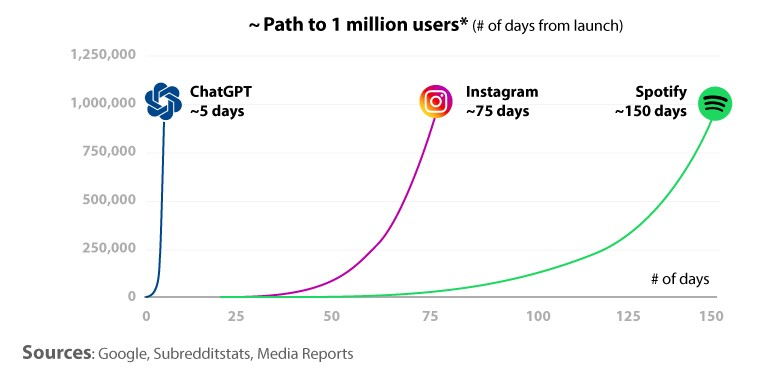
\includegraphics[width=.8\linewidth]{figures/fig0-chatgpt-growth.jpg}
\end{frame}

\begin{frame}{2024 год: Нобелевские премии за нейросети}
    \centering
    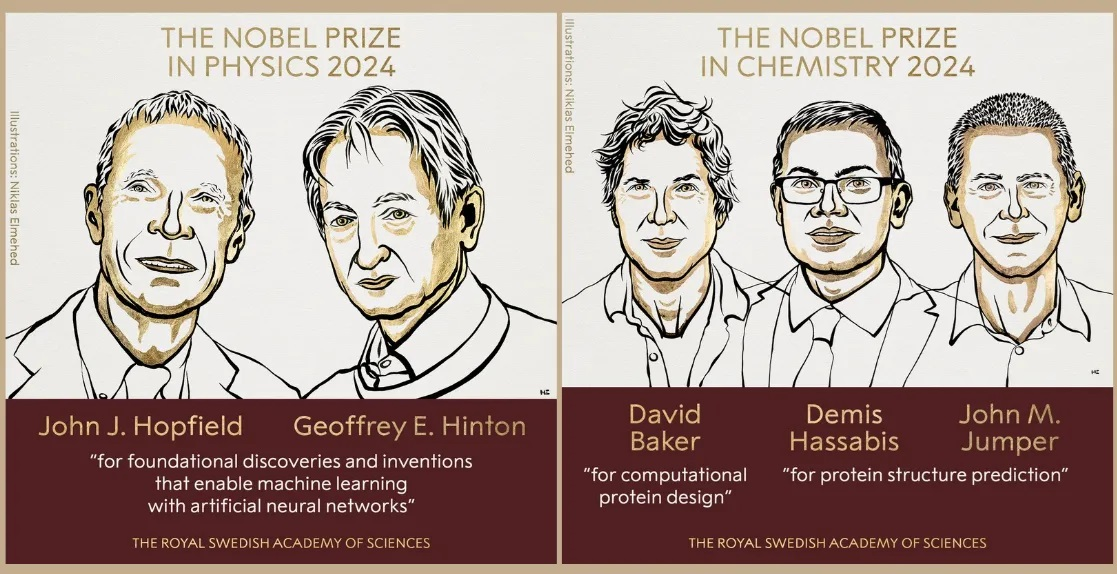
\includegraphics[width=.85\linewidth]{figures/fig1-2024-nobel-prize.jpg}
\end{frame}

\begin{frame}{2024 год: ядерные реакторы для датацентров}
    \centering
    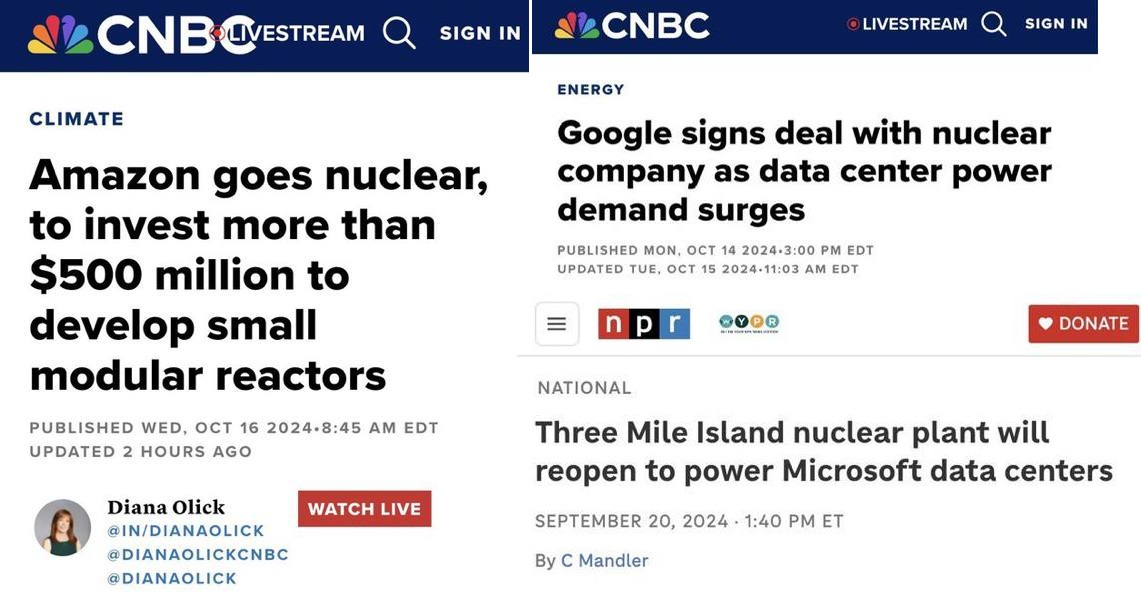
\includegraphics[width=.85\linewidth]{figures/fig2-news.jpg}
\end{frame}

\begin{frame}{Как термины связаны между собой?}
    \centering
    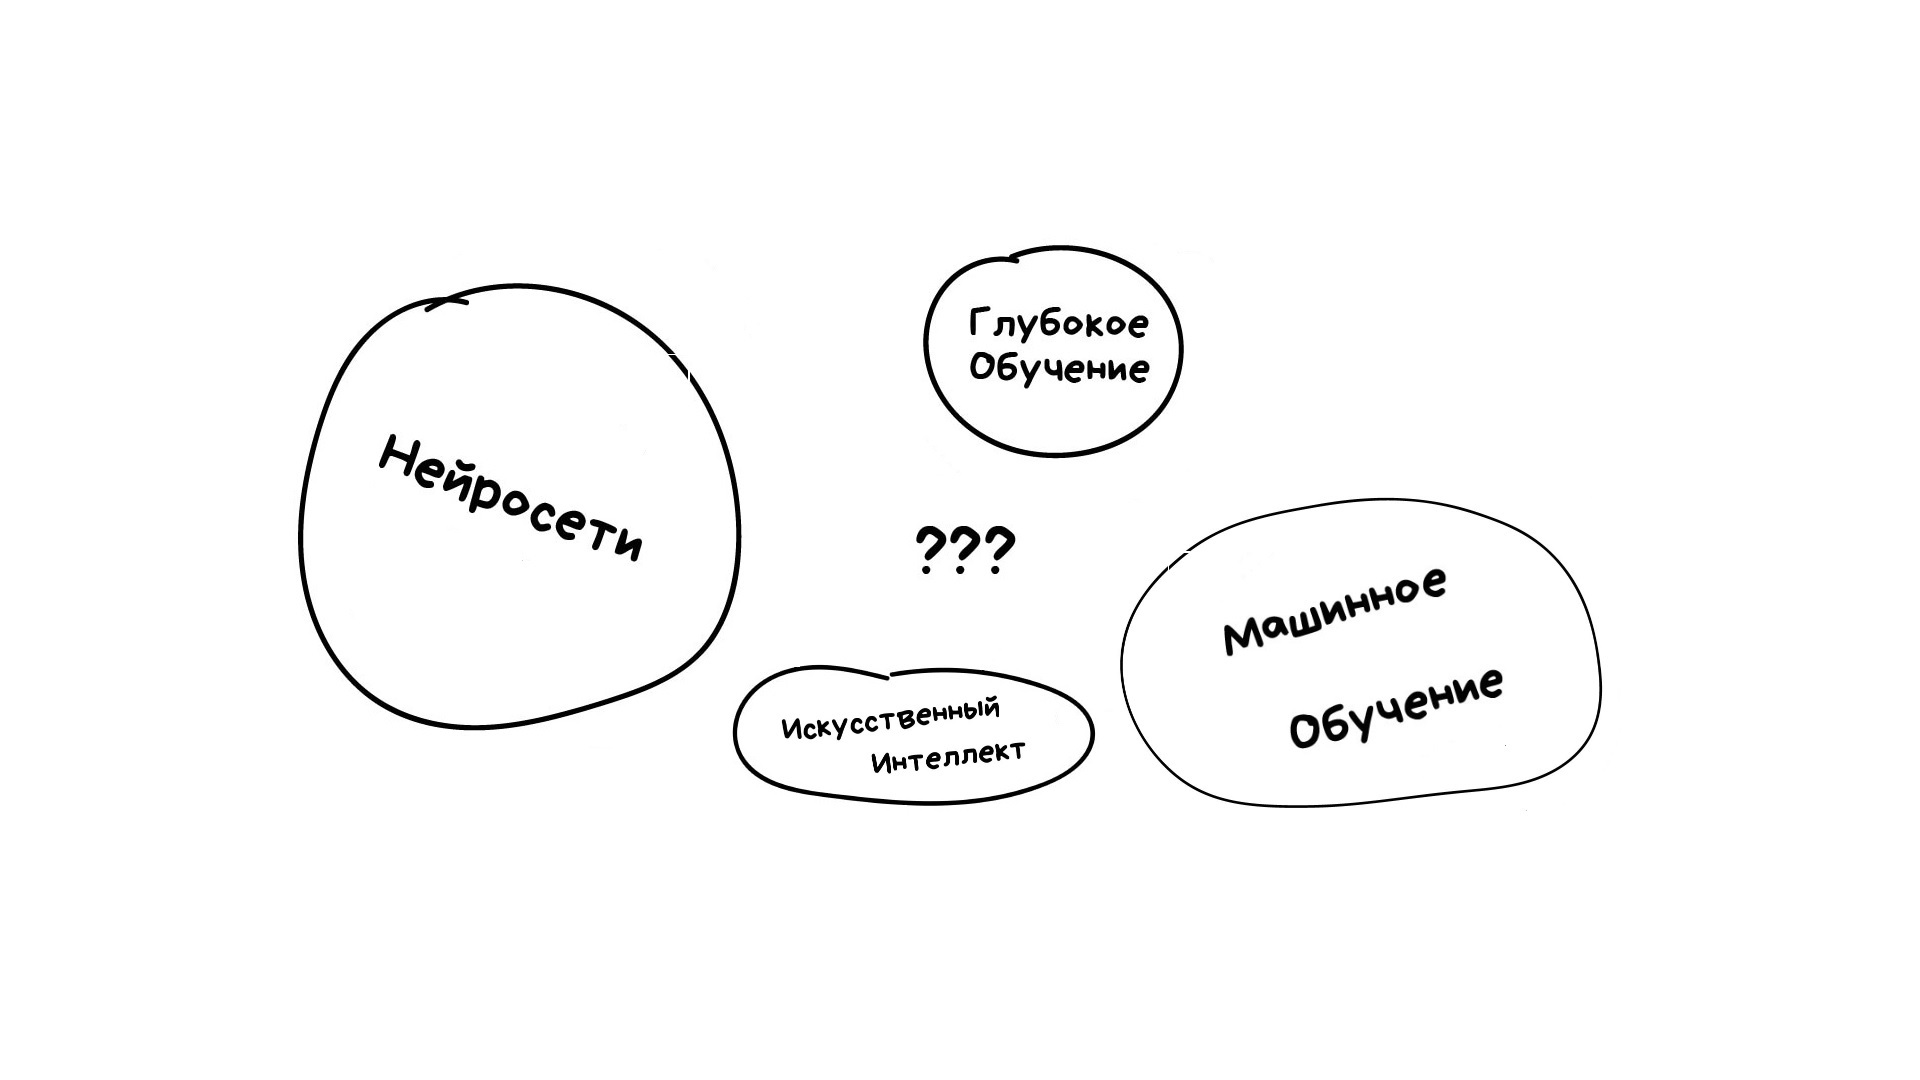
\includegraphics[width=.85\linewidth]{figures/fig3-terms.jpg}
\end{frame}

\begin{frame}{Определения: AI}
    Искусcтвенный интеллект (ИИ, AI) --- область науки, изучающая построение вычислимых
    алгоритмов для решения задач, которые люди каким-то образом решают,
    но которые сходу непонятно как автоматизировать.\\
    Например:
    \begin{outline}
        \1 корректный перевод с одного языка на другой
        \1 определение объектов на изображении
        \1 постановка диагноза по симптомам
        \1 рекомендация фильма на вечер
        \1 управление автомобилем
        \1 ...
    \end{outline}

    Иногда используют термин "когнитивные задачи".
\end{frame}

\begin{frame}{Определения: AI}
    Разделяют сильный (strong, general, AGI) и слабый (weak) AI:
    \begin{columns}
        \begin{column}{.35\linewidth}
            \centering
            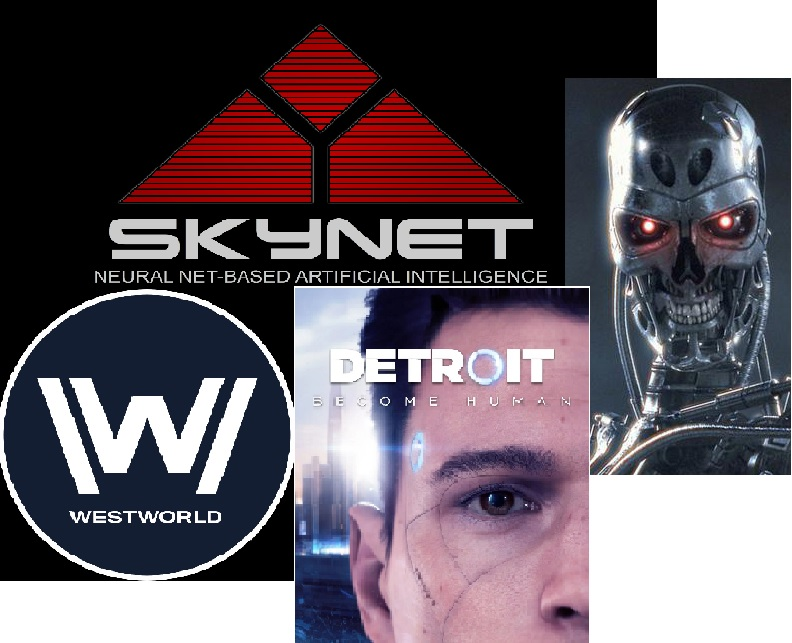
\includegraphics[width=\linewidth]{figures/fig4-strong-ai.jpg}
            Сильный ИИ \\
            \footnotesize{захватывает человечество}
        \end{column}

        \begin{column}{.35\linewidth}
            \centering
            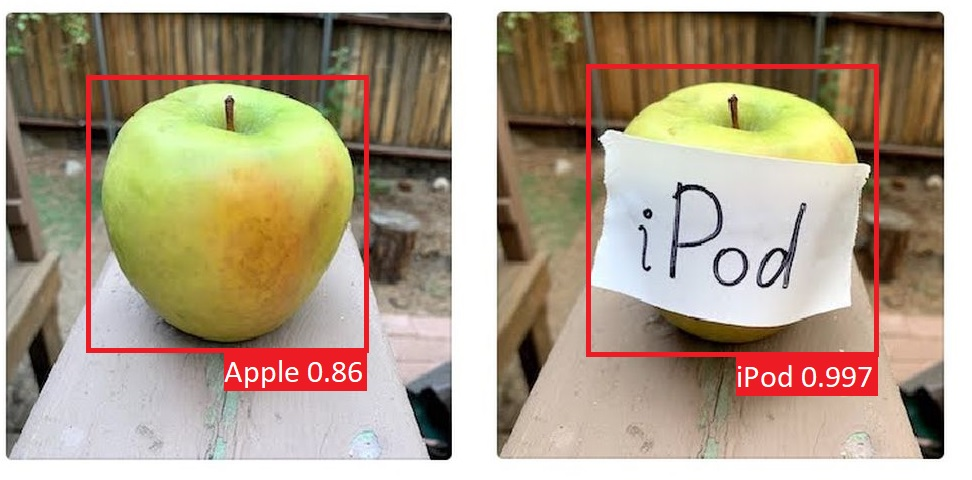
\includegraphics[width=\linewidth]{figures/fig5-weak-ai.jpg}
            Слабый ИИ \\
            \footnotesize{невероятно наивен}
        \end{column}
    \end{columns}
\end{frame}

\begin{frame}{Определения: AI}
    Разделяют сильный (strong, general, AGI) и слабый (weak) AI:
    \begin{columns}
        \begin{column}{.35\linewidth}
            \centering
            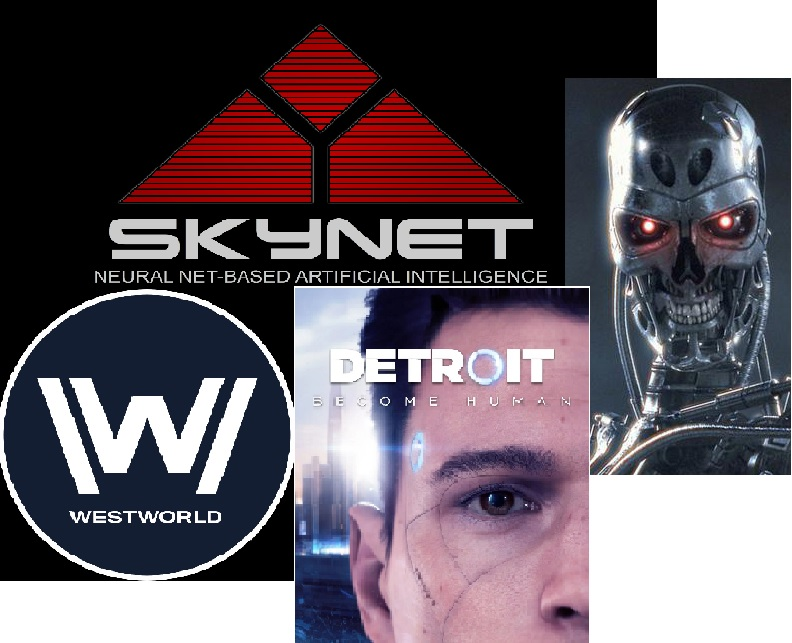
\includegraphics[width=\linewidth]{figures/fig4-strong-ai.jpg}
            Сильный ИИ \\
            \footnotesize{автономен, может заменить человека}
        \end{column}
        \begin{column}{.35\linewidth}
            \centering
            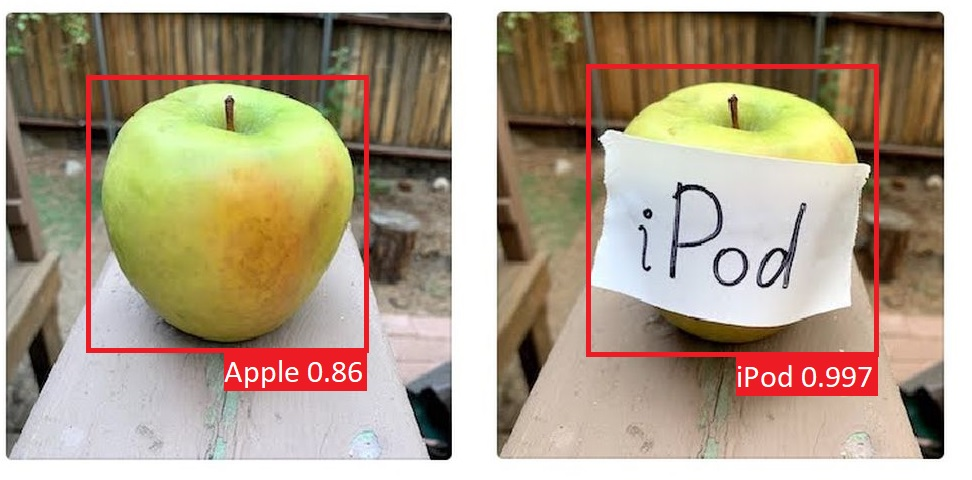
\includegraphics[width=\linewidth]{figures/fig5-weak-ai.jpg}
            Слабый ИИ \\
            \footnotesize{решает одну узкую задачу}
        \end{column}
    \end{columns}
\end{frame}


\begin{frame}{Определения: ML, NN}
    \begin{outline}
        \1 Машинное обучение (ML) --- область искусственного интеллекта, изучающая алгоритмы,
        автоматически улучшающися благодаря опыту (примерам решения задачи)
        \1 Нейронные сети --- один из множества алгоритмов машинного обучения
        \1 Глубокое обучение --- специальное название для глубоких нейронных сетей (на данный момент - практически синоним для нейронных сетей)
    \end{outline}
\end{frame}

\begin{frame}{Как термины связаны между собой?}
    \centering
    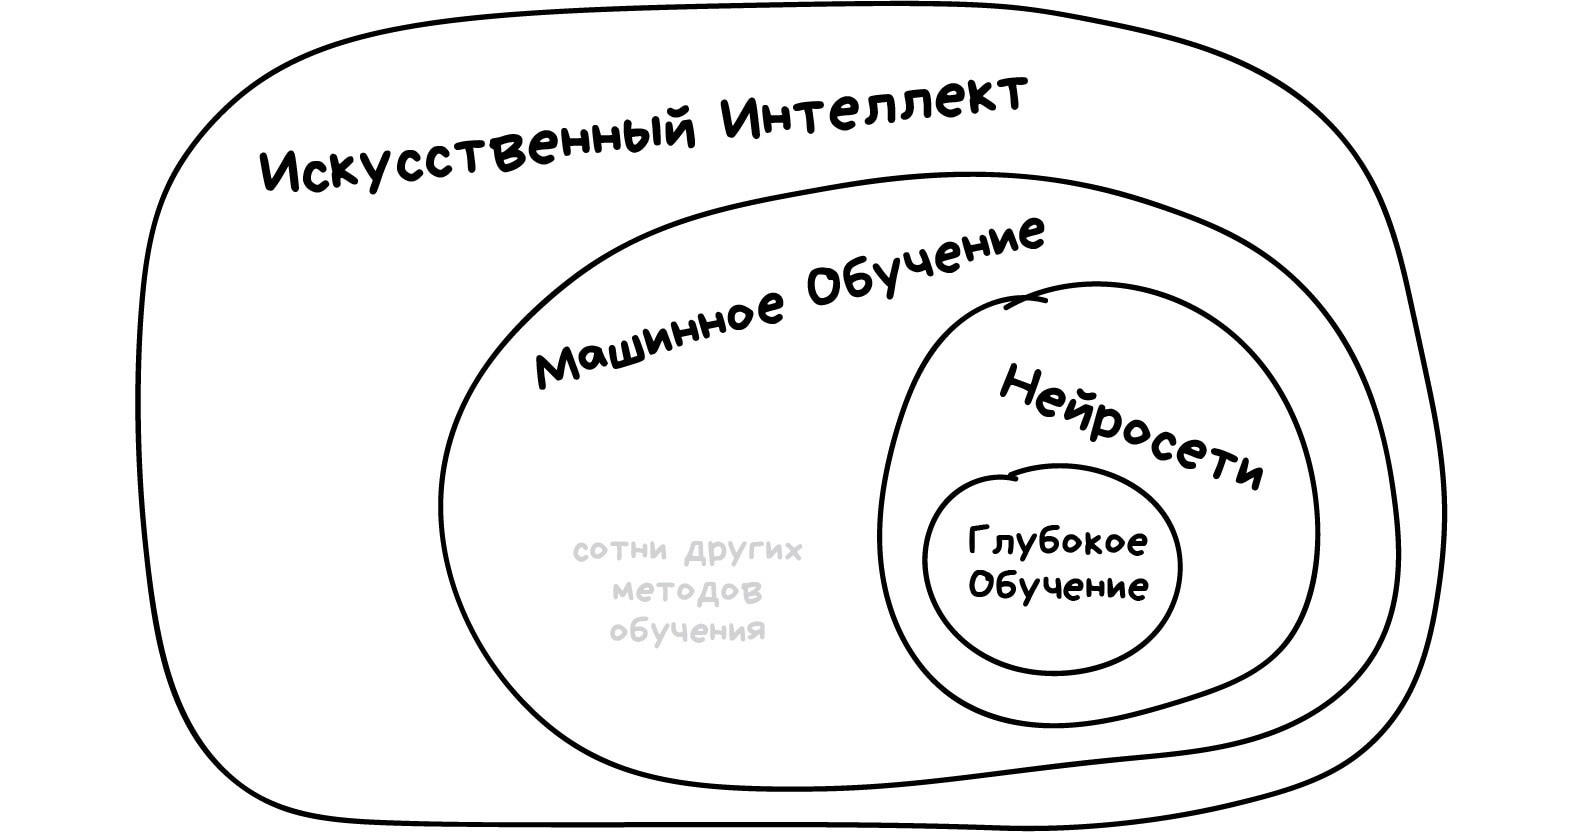
\includegraphics[width=.9\linewidth]{figures/fig6-terms.jpg}
\end{frame}

\begin{frame}{Посмотрим еще раз на задачи}
    \begin{outline}
        \1 корректный перевод с одного языка на другой
        \1 определение объектов на изображении
        \1 постановка диагноза по симптомам
        \1 рекомендация фильма на вечер
        \1 управление автомобилем
        \1 ...
    \end{outline}
\end{frame}

\begin{frame}{Что объединяет эти задачи?}
    \begin{outline}
        \1 Их решение (или часть решения) можно записать как функцию, которая отображает
        \textbf{объекты} (примеры, samples) в \textbf{предсказания} (targets)
            \2 \( f("Hello \ world!") \to \) "Привет, мир!"
            \2 \( f(netflix \ history) \to \) [Головоломка 2]
            \2 \( f(t = 37^\circ C) \to \) вы больны с вероятностью 0.5
        \pause
        \1 Можно собрать примеры правильных и неправильных решений
        \pause
        \1 Подходит не идеальное, а просто достаточно хорошее решение
            (люди тоже нередко ошибаются)
    \end{outline}

    Более подробно разберем особенности на примере задачи классификации изображений (именно с этой задачи началась популярность нейросетей)
\end{frame}

\begin{frame}{Задача классификации изображений}
    Для заданного изображения нужно найти правильную метку
    из конечного дискретного набора \( C \)
    \vfill
    \begin{columns}
        \begin{column}{.35\linewidth}
            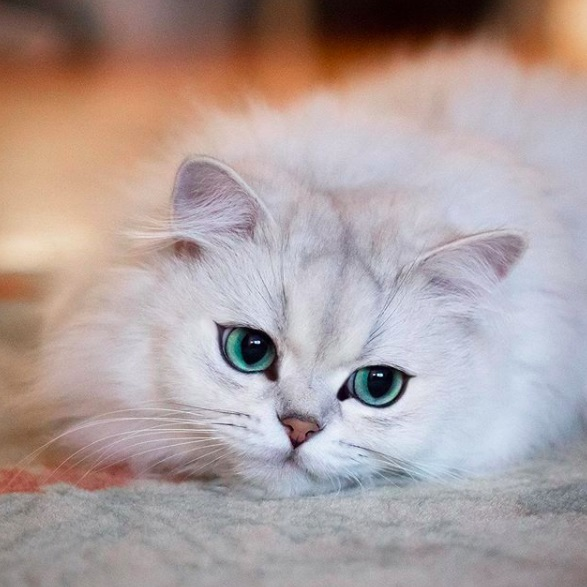
\includegraphics[width=\linewidth]{figures/fig7-cat.jpg}
        \end{column}
        \begin{column}{.65\linewidth}
            \( C = \{dog, cat, parrot, human, car, ninja, \ldots \} \) \\
            \hfill
            \vfill
            \( \Longrightarrow \quad \) cat
        \end{column}
    \end{columns}
\end{frame}

\begin{frame}{Задача классификации изображений}
    Более формально: построить функцию
    \( f(x) \rightarrow l, \quad l \in C \), \(x\) --- входное изображение
    \vfill
    \begin{columns}
        \begin{column}{.49\linewidth}
            \centering
            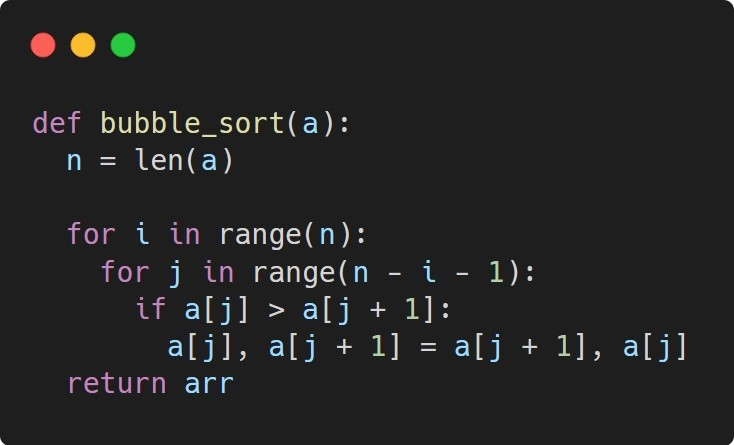
\includegraphics[width=\linewidth]{figures/fig8-bubble-sort.jpg}
            Сортировка пузырьком
        \end{column}
        \begin{column}{.43\linewidth}
            \centering
            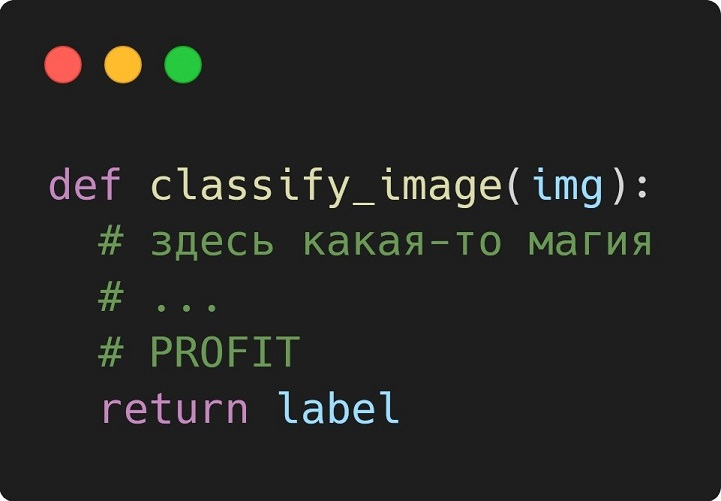
\includegraphics[width=\linewidth]{figures/fig9-clf-function.jpg}
            Классификация
        \end{column}
    \end{columns}
\end{frame}

\begin{frame}{Ученые недооценили сложность}
    \begin{columns}
        \begin{column}{.43\linewidth}
            \centering
            Ожидание в 1966
            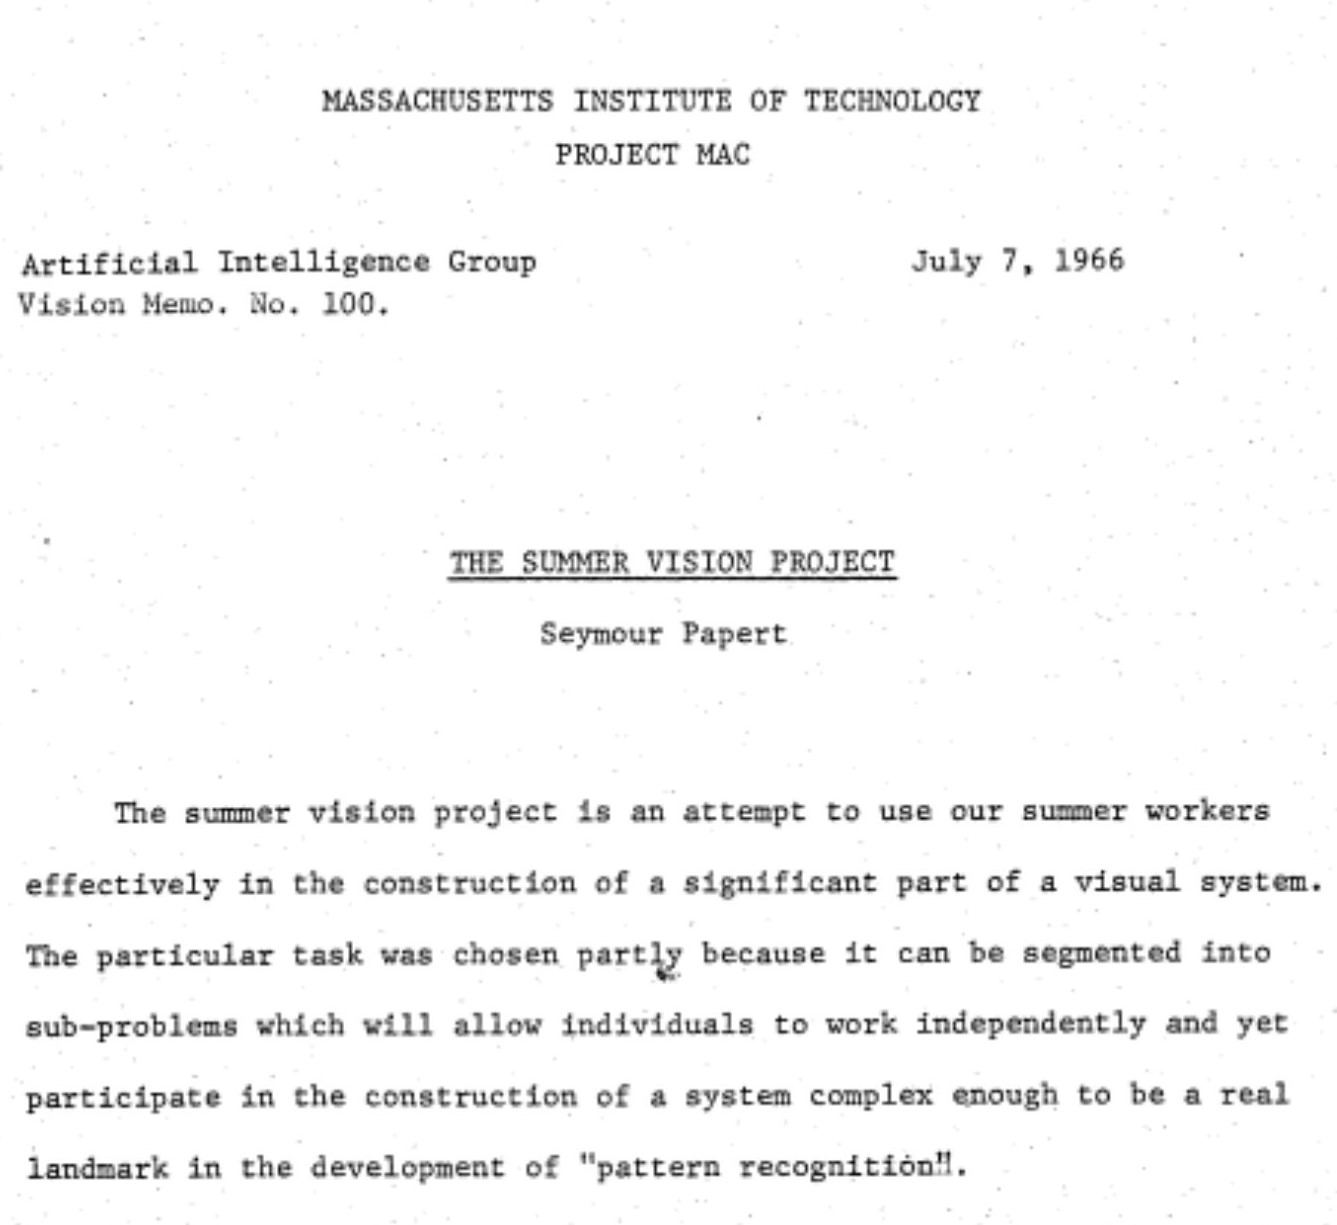
\includegraphics[width=\linewidth]{figures/fig10-summer-vision.jpg}
        \end{column}
        \pause
        \begin{column}{.24\linewidth}
            \centering
            Реальность до 2012
            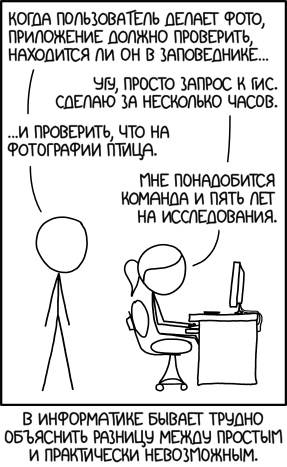
\includegraphics[width=\linewidth]{figures/fig11-xkcd-gis.jpg}
        \end{column}
    \end{columns}
\end{frame}

\begin{frame}{Ученые недооценили сложность}
    \begin{columns}
        \begin{column}{.33\linewidth}
            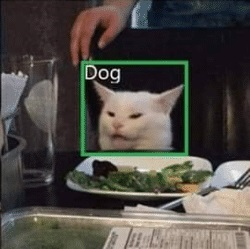
\includegraphics[width=\linewidth]{figures/fig12-error-1.jpg}
        \end{column}
        \begin{column}{.33\linewidth}
            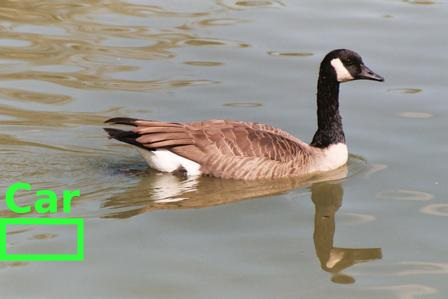
\includegraphics[width=\linewidth]{figures/fig13-error-2.jpg}
        \end{column}
        \begin{column}{.33\linewidth}
            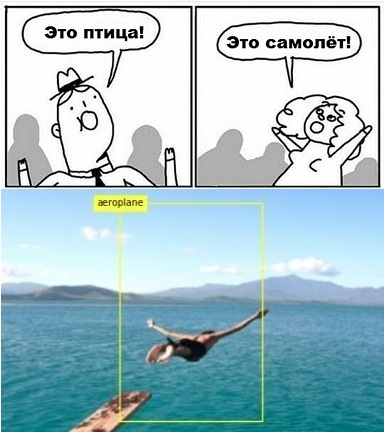
\includegraphics[width=\linewidth]{figures/fig14-error-3.jpg}
        \end{column}
    \end{columns}
\end{frame}

\begin{frame}{Семантический разрыв (semantic gap)}
    \begin{columns}
        \begin{column}{.35\linewidth}
            \centering
            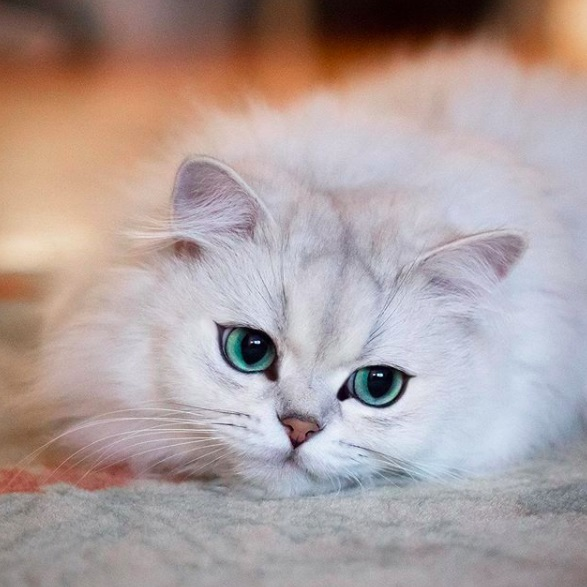
\includegraphics[width=\linewidth]{figures/fig7-cat.jpg}
            Мы: кошка
        \end{column}
        \begin{column}{.65\linewidth}
            \centering
            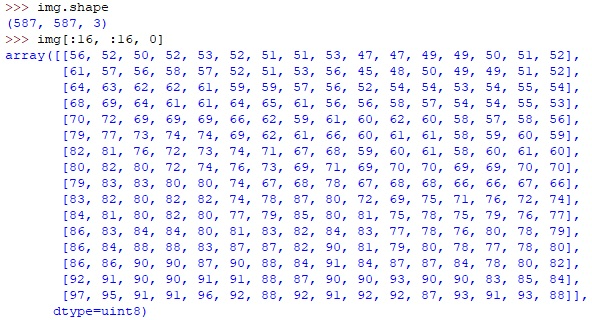
\includegraphics[width=\linewidth]{figures/fig15-rgb.jpg}
            Компьютер: какая кошка?
        \end{column}
    \end{columns}
\end{frame}

\begin{frame}{Смена ракурса}
    \begin{columns}
        \begin{column}{.325\linewidth}
            \centering
            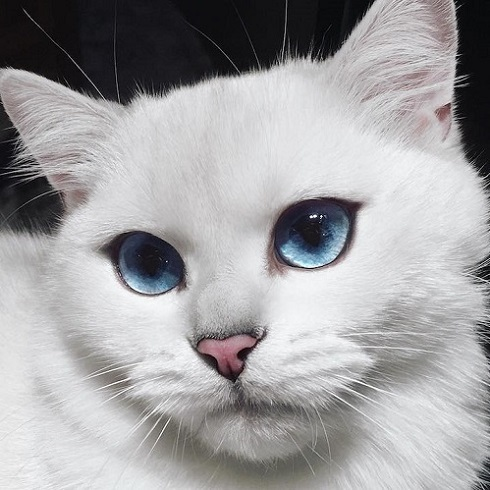
\includegraphics[width=\linewidth]{figures/fig16-cat.jpg}
        \end{column}
        \begin{column}{.325\linewidth}
            \centering
            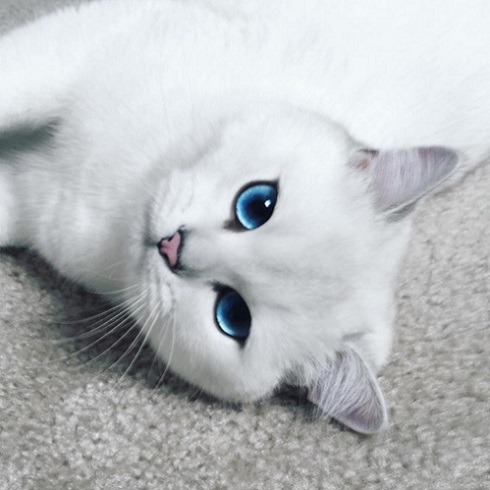
\includegraphics[width=\linewidth]{figures/fig17-cat.jpg}
        \end{column}
        \begin{column}{.325\linewidth}
            \centering
            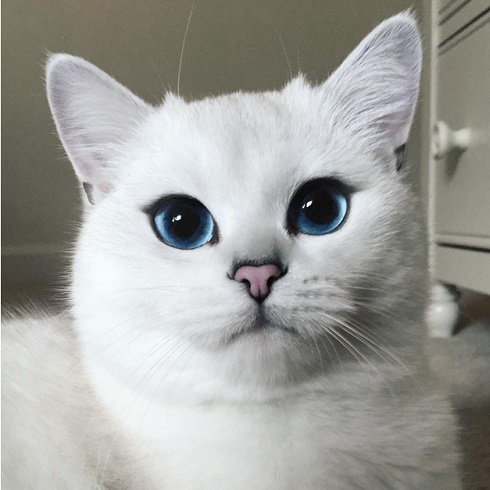
\includegraphics[width=\linewidth]{figures/fig18-cat.jpg}
        \end{column}
    \end{columns}
    \begin{center}
        Меняются практически все пиксели изображения
    \end{center}
\end{frame}

\begin{frame}{Разное освещение}
    \begin{columns}
        \begin{column}{.25\linewidth}
            \centering
            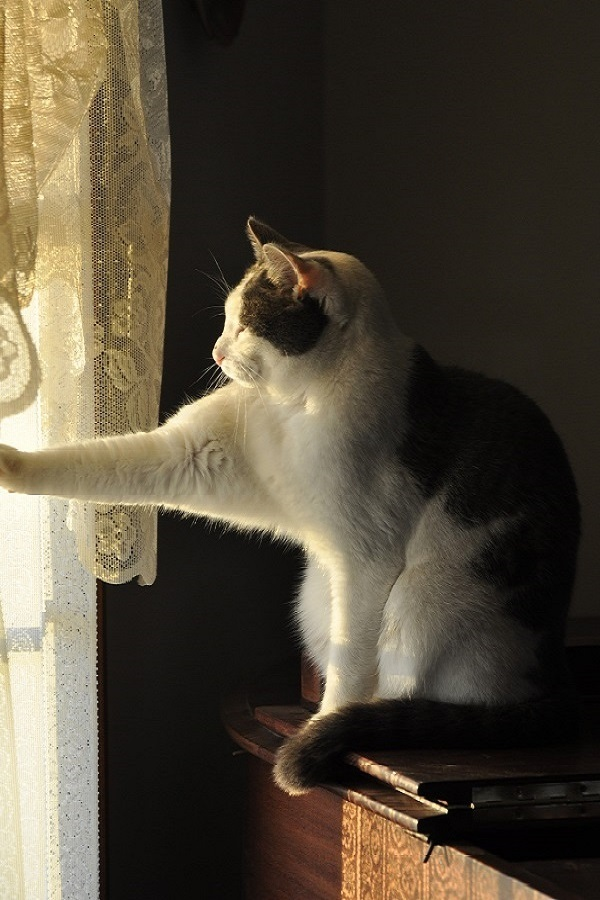
\includegraphics[width=\linewidth]{figures/fig19-cat.jpg}
        \end{column}
        \begin{column}{.25\linewidth}
            \centering
            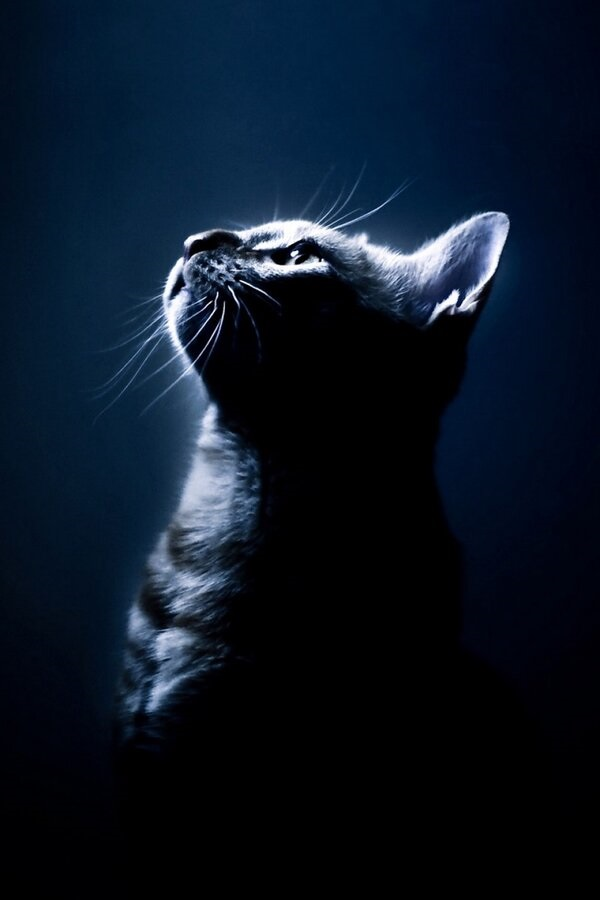
\includegraphics[width=\linewidth]{figures/fig20-cat.jpg}
        \end{column}
        \begin{column}{.25\linewidth}
            \centering
            
\includegraphics[width=\linewidth]{figures/fig21-cat.jpg}
        \end{column}
    \end{columns}
    \begin{center}
        Меняются практически все пиксели изображения
    \end{center}
\end{frame}

\begin{frame}{Вариация форм (коты жидкие)}
    \begin{columns}
        \begin{column}{.25\linewidth}
            \centering
            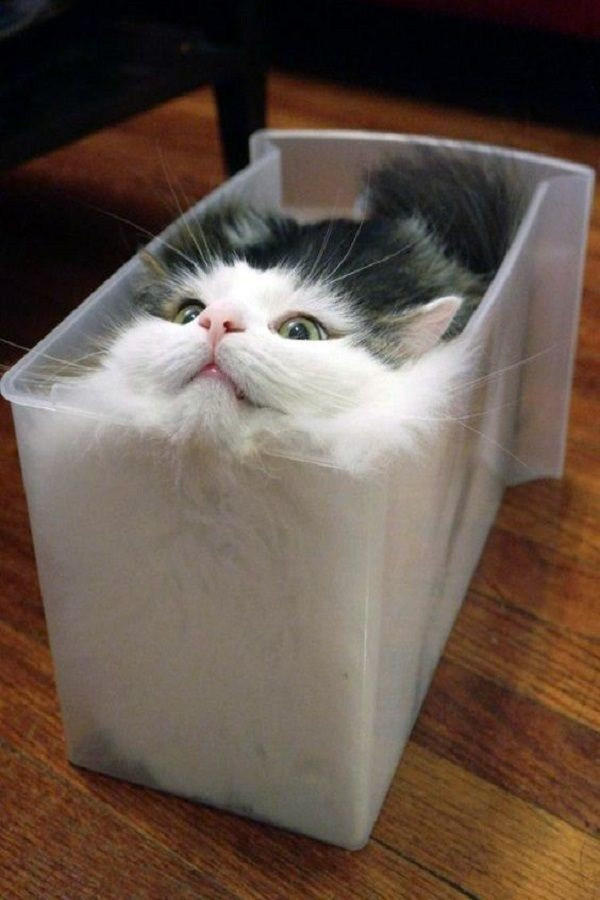
\includegraphics[width=\linewidth]{figures/fig22-cat.jpg}
        \end{column}
        \begin{column}{.25\linewidth}
            \centering
            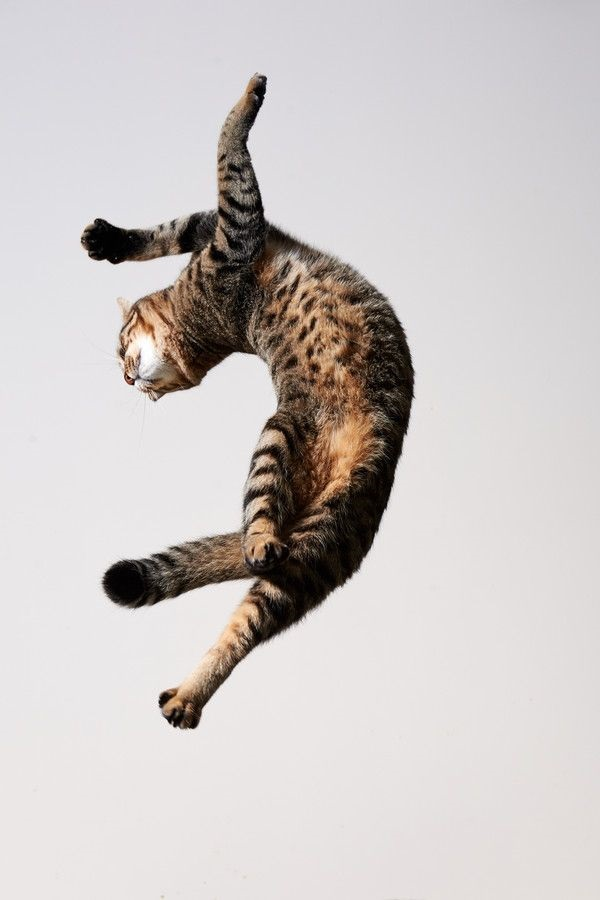
\includegraphics[width=\linewidth]{figures/fig23-cat.jpg}
        \end{column}
        \begin{column}{.25\linewidth}
            \centering
            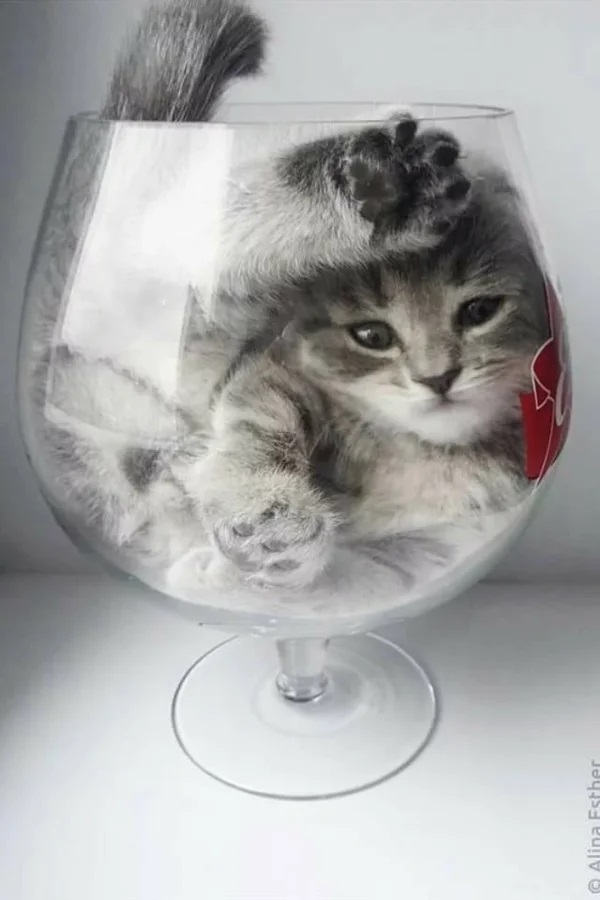
\includegraphics[width=\linewidth]{figures/fig24-cat.jpg}
        \end{column}
    \end{columns}
    \begin{center}
        Меняются практически все пиксели изображения
    \end{center}
\end{frame}

\begin{frame}{Внутриклассовая вариативность}
    \centering
    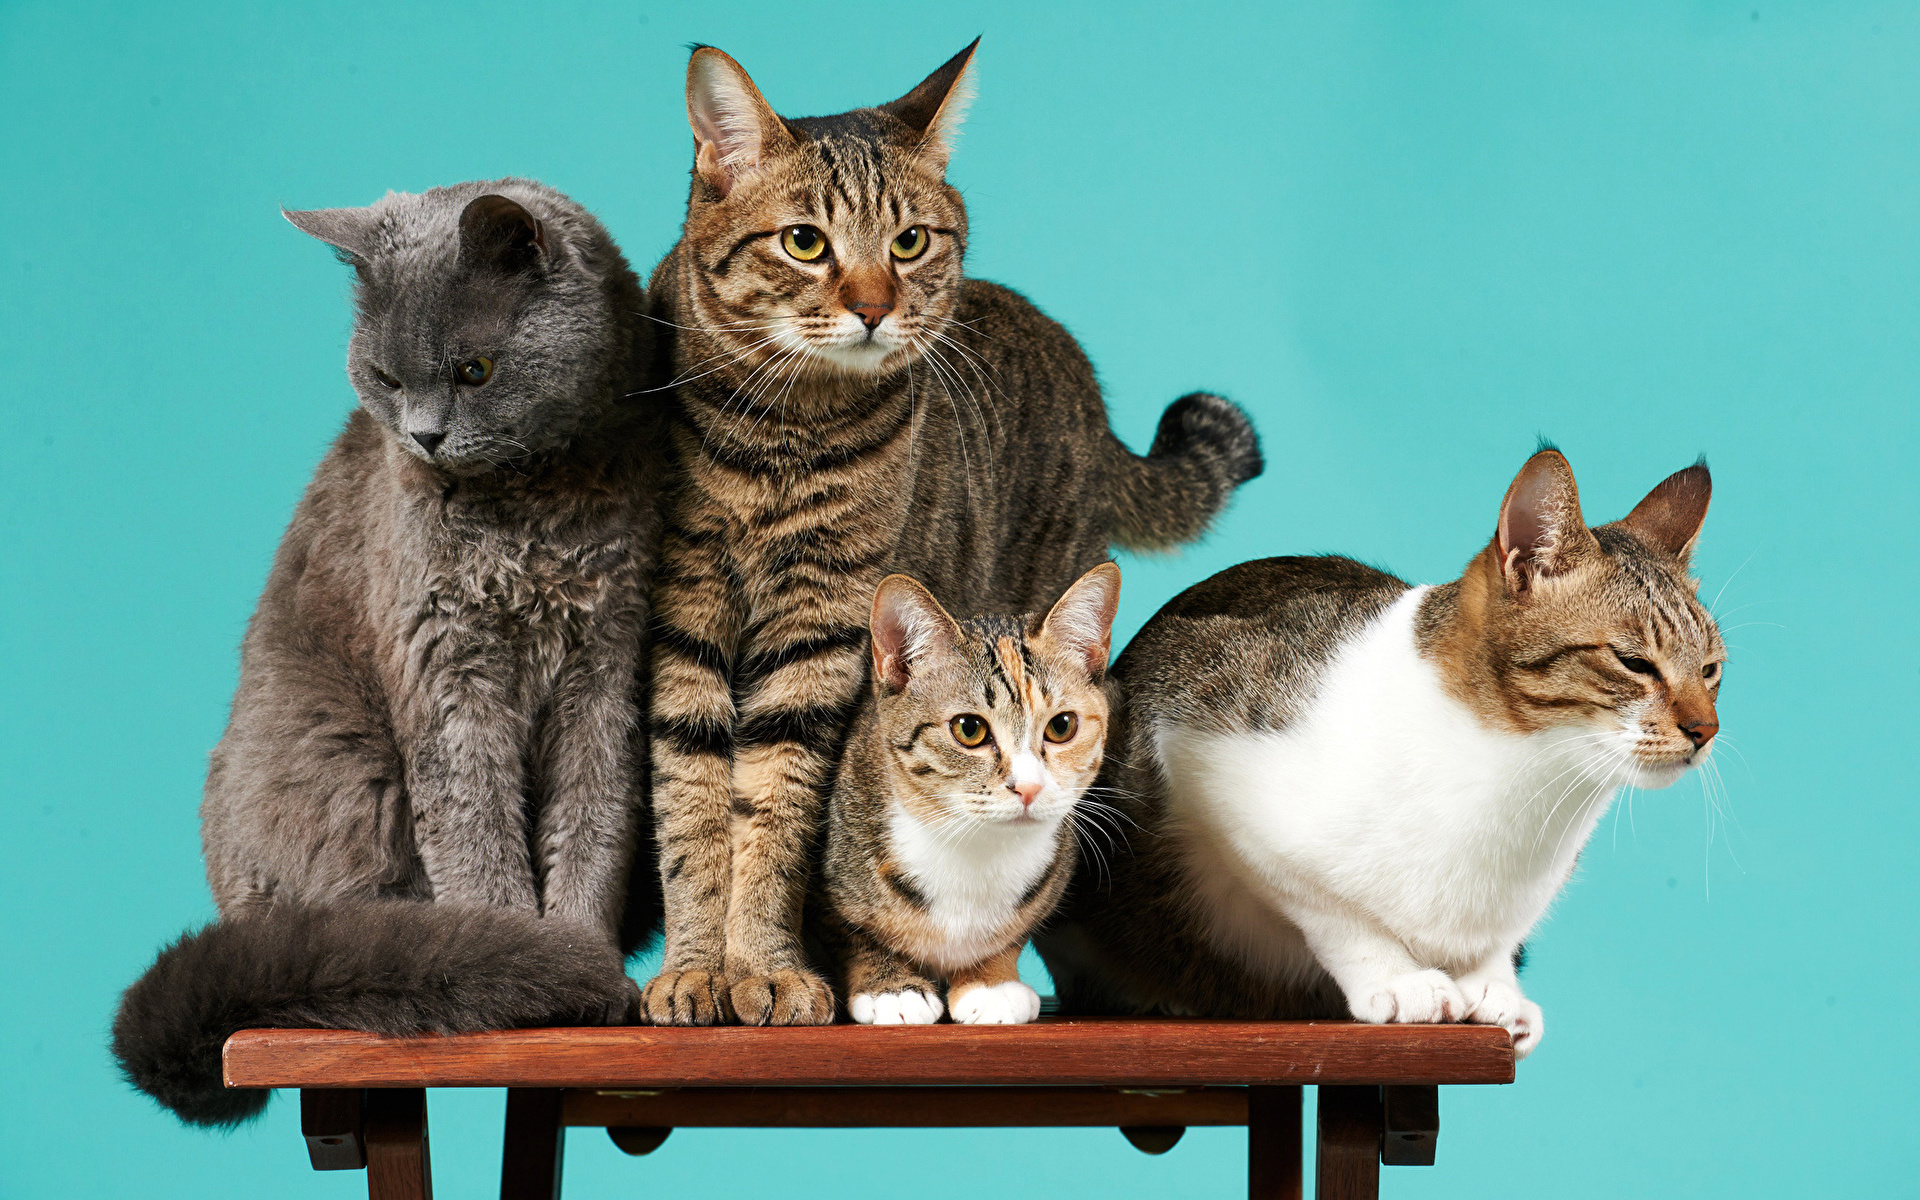
\includegraphics[width=.77\linewidth]{figures/fig25-cats.jpg}
\end{frame}

\begin{frame}{Поражение детерминированных алгоритмов}
    \centering
    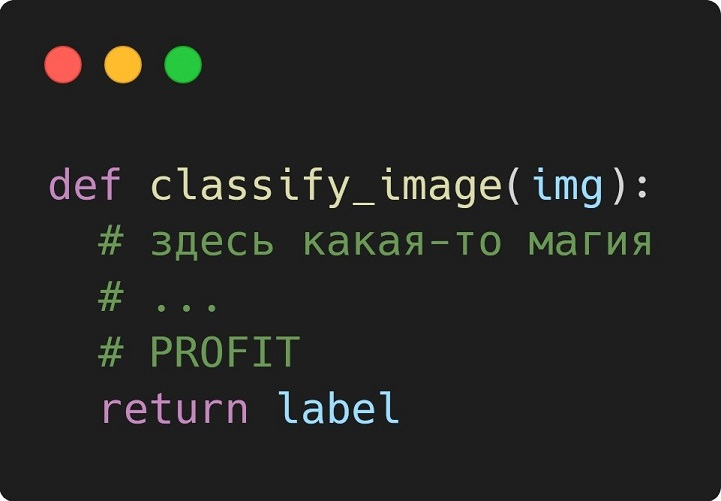
\includegraphics[width=.5\linewidth]{figures/fig9-clf-function.jpg}

    \textbf{Простого} способа построить такую функцию так и не нашлось
\end{frame}

\begin{frame}{Поражение детерминированных алгоритмов}
    Было предпринято множество попыток, однако они работали только в ограниченном
    числе случаев и переставали работать при изменении условий
    \vfill
    \begin{columns}
        \begin{column}{.25\linewidth}
            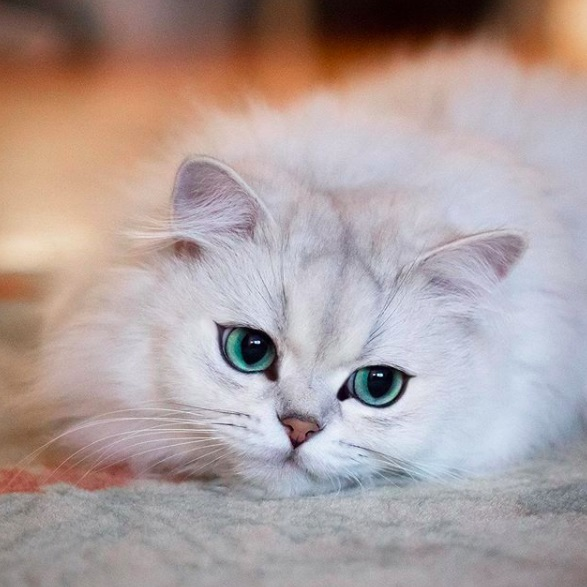
\includegraphics[width=\linewidth]{figures/fig7-cat.jpg}
        \end{column}
        \begin{column}{.15\linewidth}
            \centering
            \( \longrightarrow \) \\
            границы
        \end{column}
        \begin{column}{.25\linewidth}
            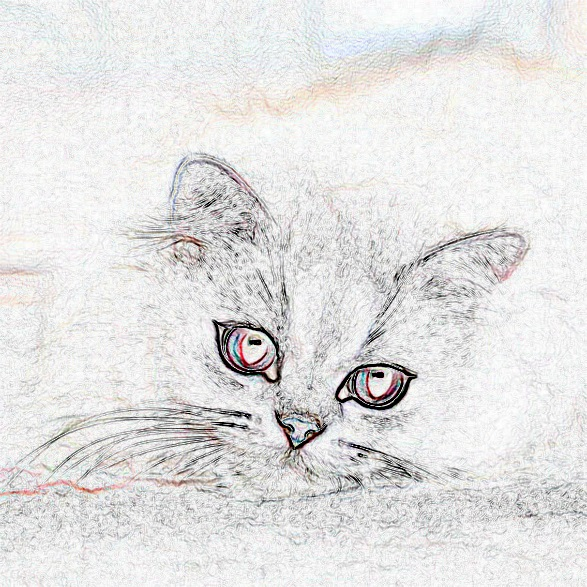
\includegraphics[width=\linewidth]{figures/fig26-cat-filtered.jpg}
        \end{column}
        \begin{column}{.15\linewidth}
            \centering
            \( \longrightarrow \) \\
            углы
        \end{column}
        \begin{column}{.07\linewidth}
            
\includegraphics[width=\linewidth]{figures/fig27-corners.jpg}
        \end{column}
        \begin{column}{.13\linewidth}
            \centering
            \( \longrightarrow  \) \\
            \(? \)
        \end{column}
    \end{columns}
\end{frame}

\begin{frame}{A wild data driven machine learning appears}
    \centering
    
\includegraphics[width=.73\linewidth]{figures/fig28-iron-man.jpg}
\end{frame}

\begin{frame}{Машинное обучение: data driven approach}
    \begin{outline}
        \1 Машинное обучение изучает алгоритмы, улучшающися благодаря опыту
        \1 Функция решения задачи --- \textbf{модель}
        \1 Набор примеров --- \textbf{обучающия выборка, датасет}
            \2 объекты (\textbf{семплы}) + ответы (\textbf{таргеты})
    \end{outline}
    \begin{columns}
        \begin{column}{.1\linewidth}
            \centering
            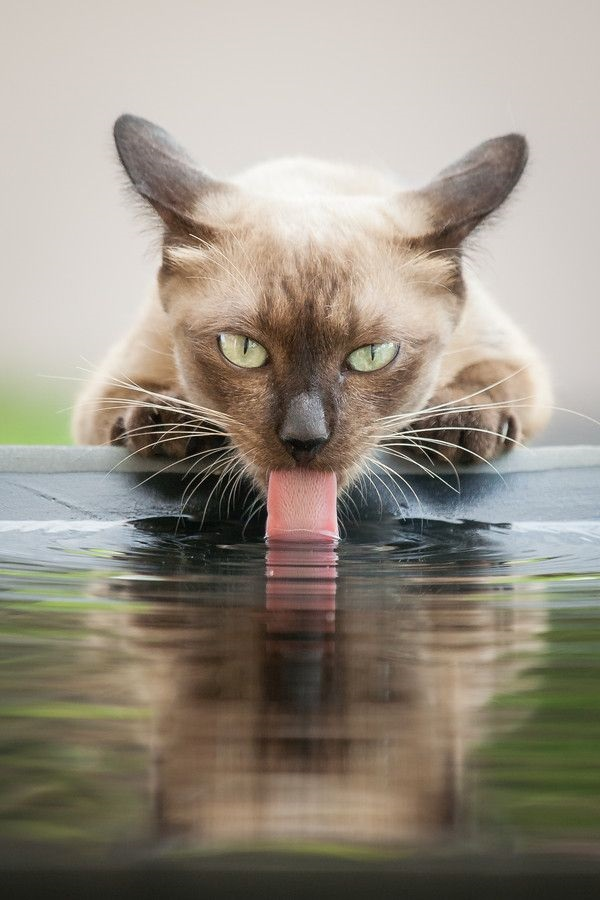
\includegraphics[width=\linewidth]{figures/fig29-dataset-sample.jpg}
            `cat'
        \end{column}
        \begin{column}{.1\linewidth}
            \centering
            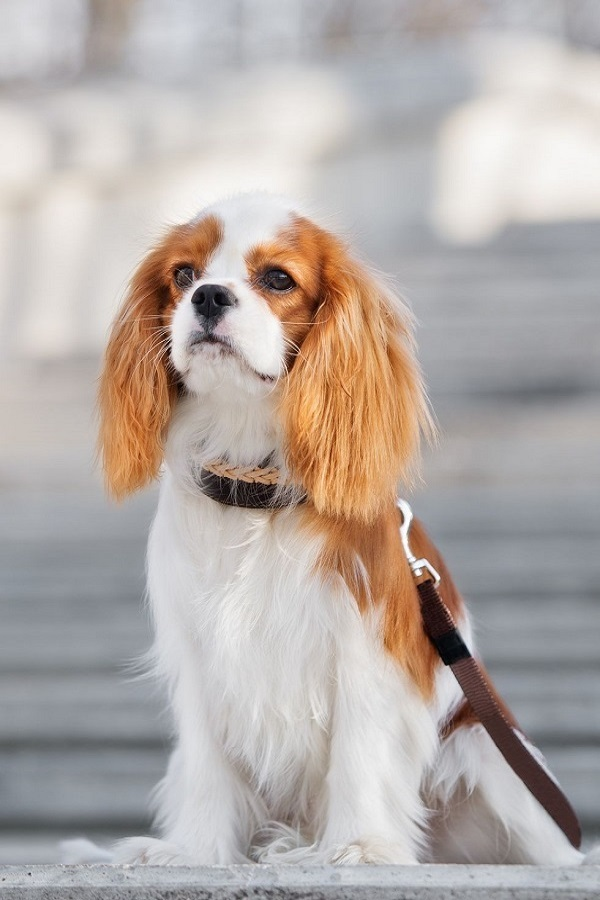
\includegraphics[width=\linewidth]{figures/fig30-dataset-sample.jpg}
            `dog'
        \end{column}
        \begin{column}{.1\linewidth}
            \centering
            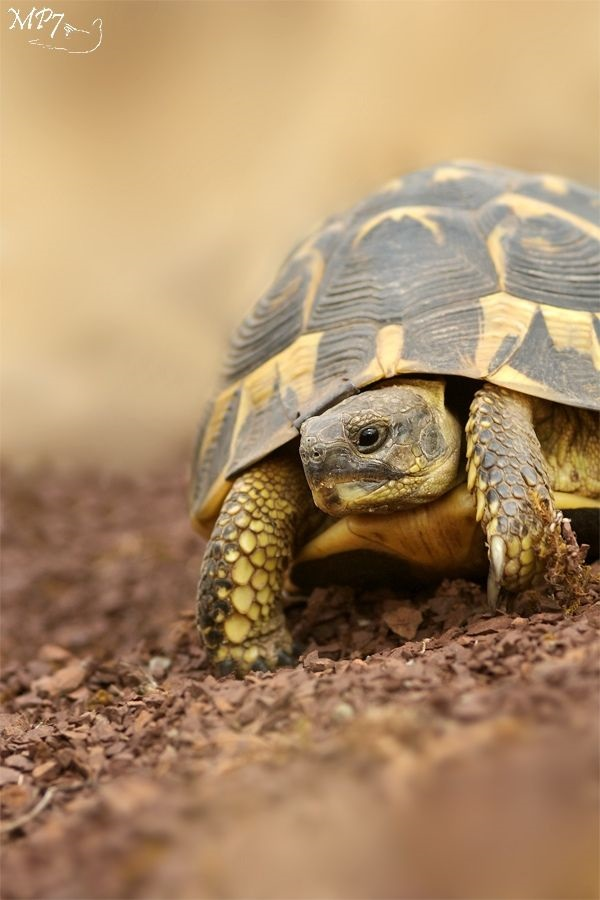
\includegraphics[width=\linewidth]{figures/fig31-dataset-sample.jpg}
            `ninja'
        \end{column}
        \begin{column}{.1\linewidth}
            \centering
            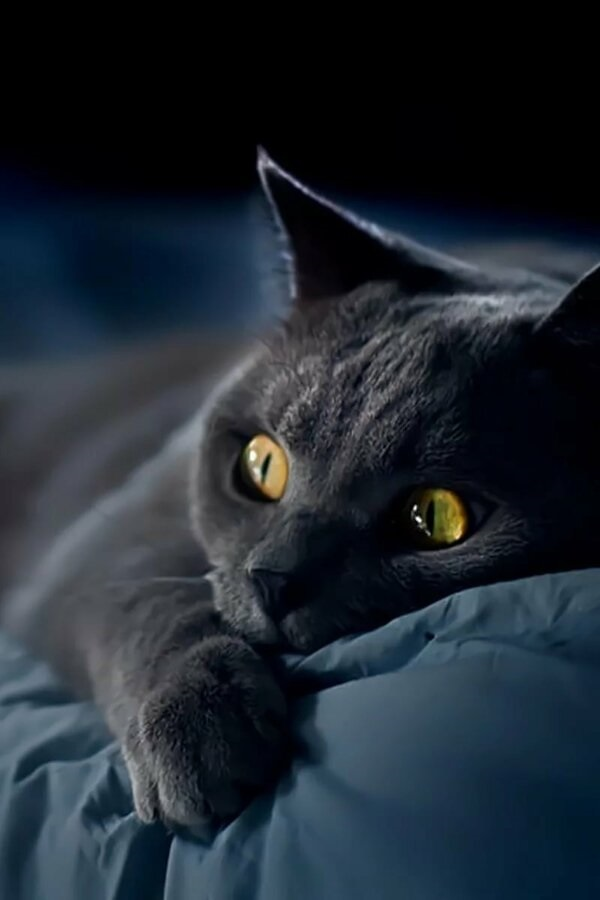
\includegraphics[width=\linewidth]{figures/fig32-dataset-sample.jpg}
            `cat'
        \end{column}
        \begin{column}{.1\linewidth}
            \centering
            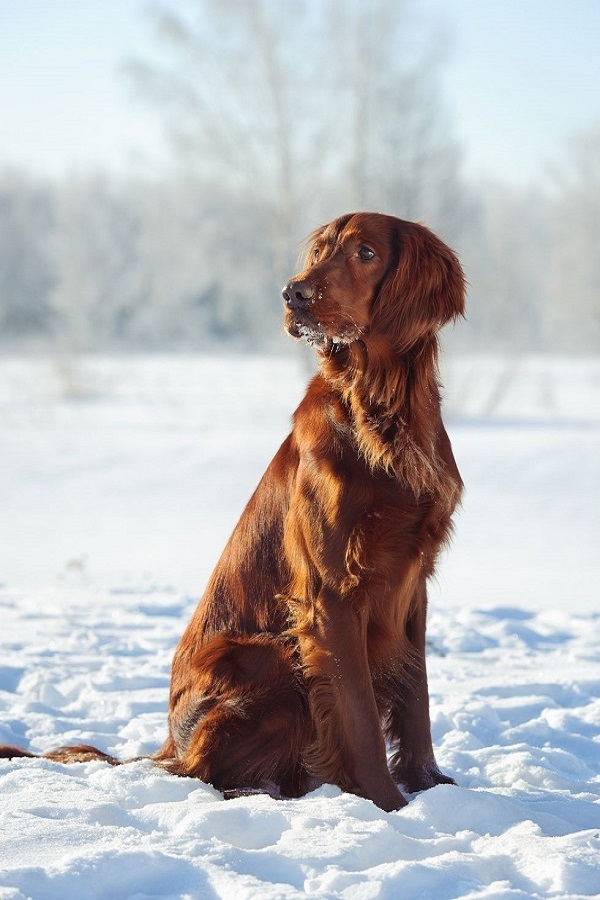
\includegraphics[width=\linewidth]{figures/fig33-dataset-sample.jpg}
            `dog'
        \end{column}
        \begin{column}{.1\linewidth}
            \centering
            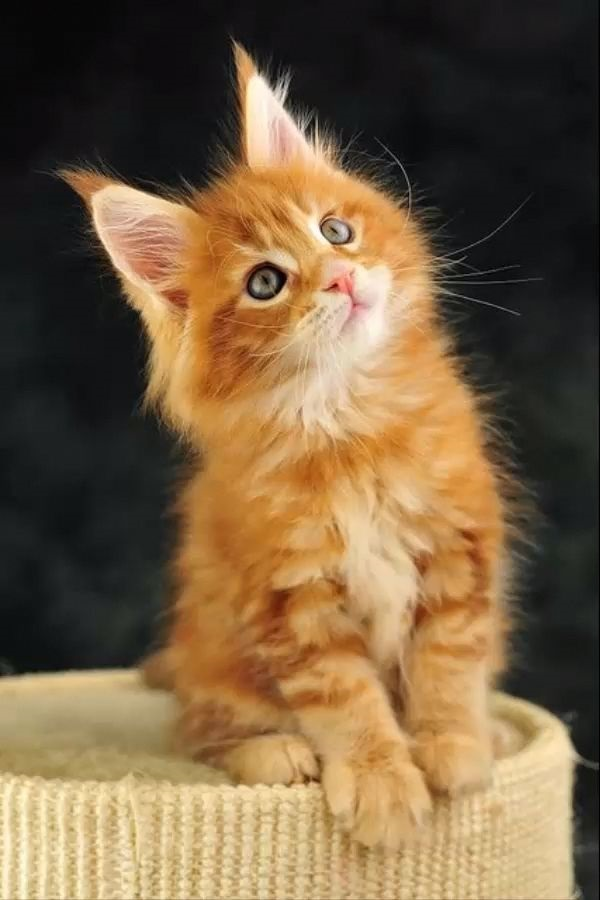
\includegraphics[width=\linewidth]{figures/fig34-dataset-sample.jpg}
            `cat'
        \end{column}
        \begin{column}{.1\linewidth}
            \centering
            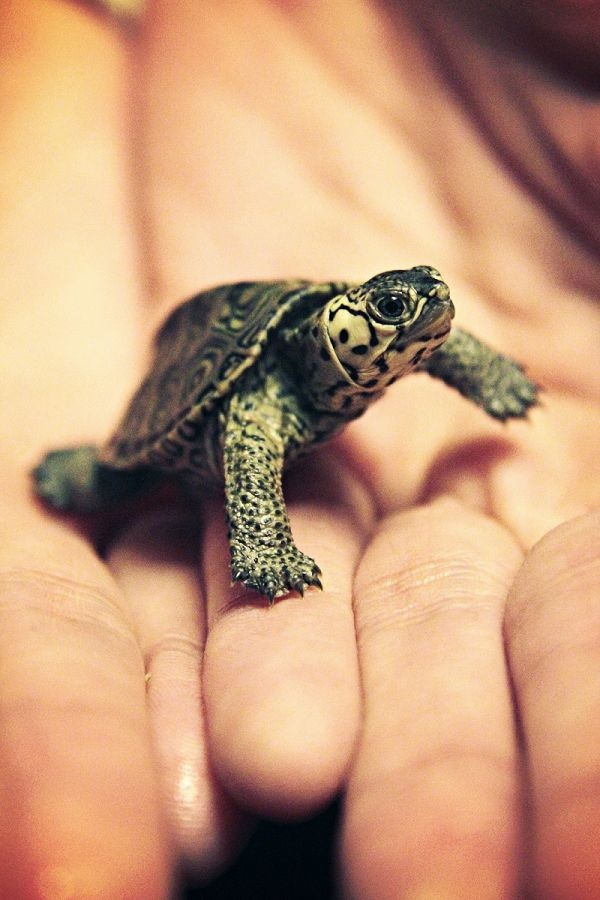
\includegraphics[width=\linewidth]{figures/fig35-dataset-sample.jpg}
            `ninja'
        \end{column}
        \begin{column}{.1\linewidth}
            \centering
            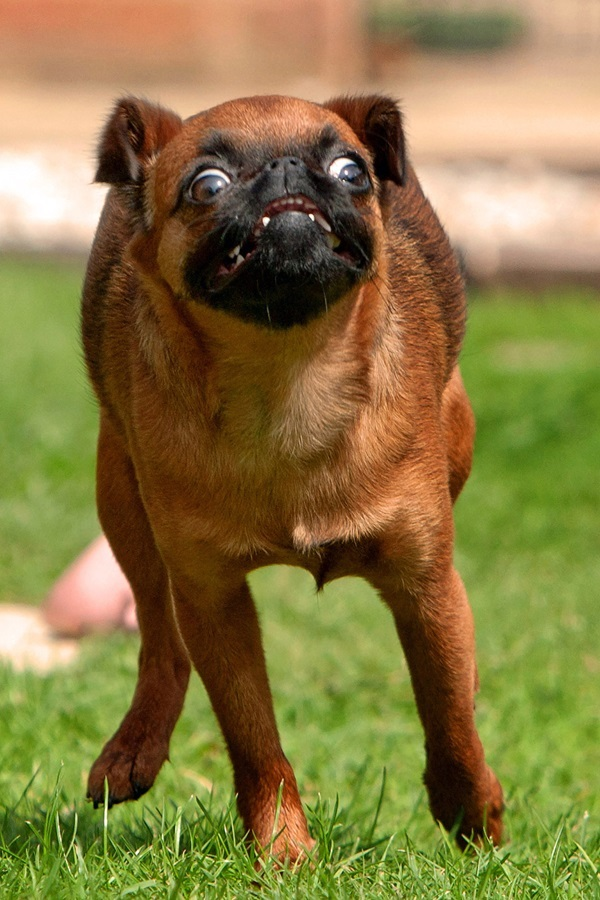
\includegraphics[width=\linewidth]{figures/fig36-dataset-sample.jpg}
            `dog'
        \end{column}
        \begin{column}{.1\linewidth}
            \centering
            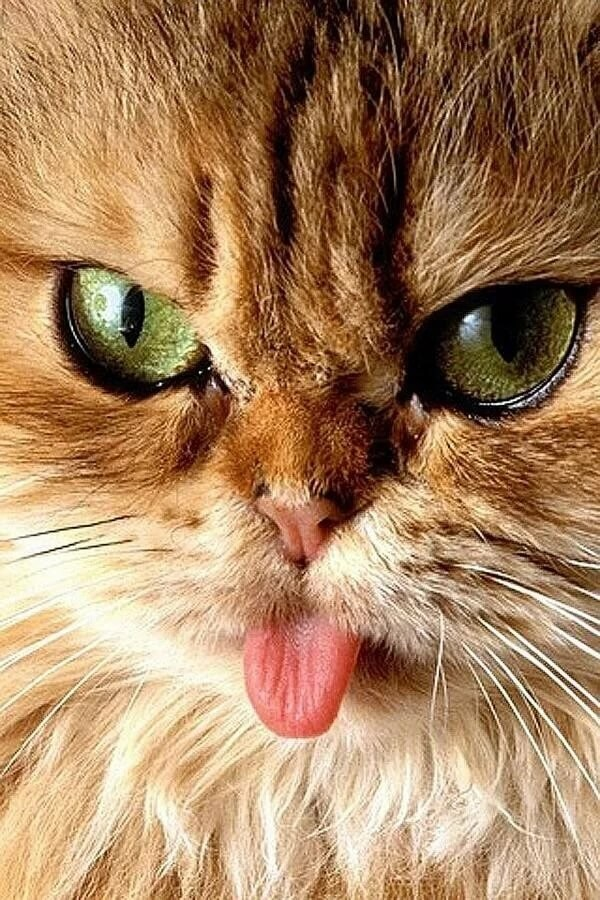
\includegraphics[width=\linewidth]{figures/fig37-dataset-sample.jpg}
            `cat'
        \end{column}
    \end{columns}
\end{frame}

\begin{frame}{Машинное обучение: data driven approach}
    \centering
    Теперь наша функция превращается в две:
    \begin{columns}[T]
        \begin{column}{.4\linewidth}
            \centering
            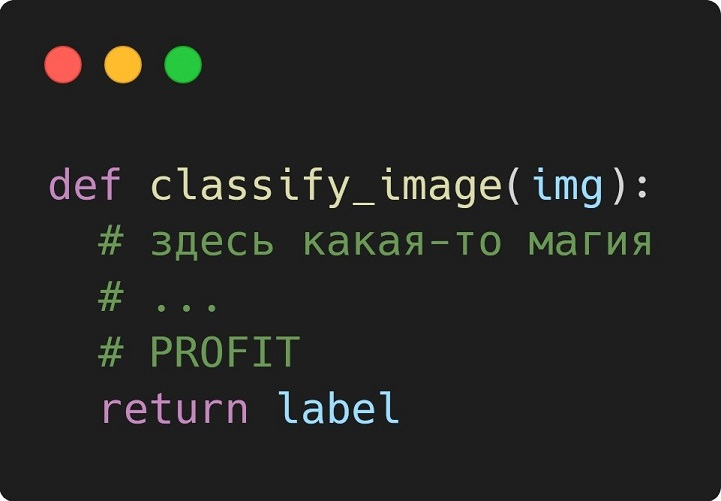
\includegraphics[width=\linewidth]{figures/fig9-clf-function.jpg}
        \end{column}
        \begin{column}{.6\linewidth}
            \centering
            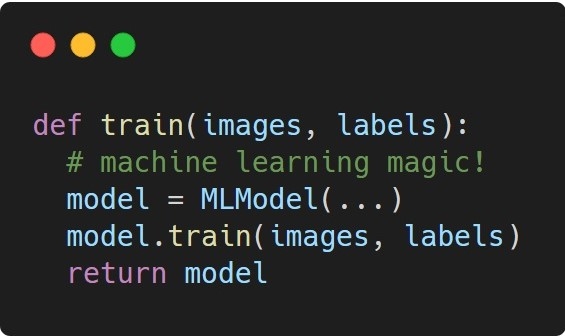
\includegraphics[width=.64\linewidth]{figures/fig38-train-func.jpg}
            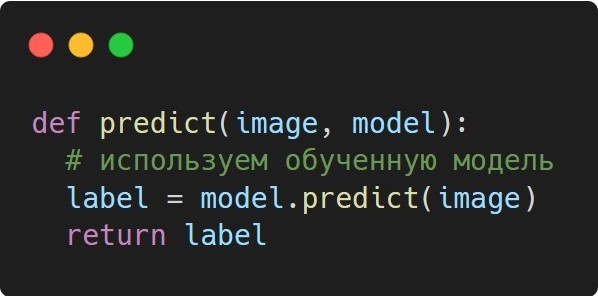
\includegraphics[width=.64\linewidth]{figures/fig39-predict-func.jpg}
        \end{column}
    \end{columns}
\end{frame}

\begin{frame}{Software Engineering vs. Machine Learning}
    \begin{columns}[T]
        \begin{column}{.49\linewidth}
            \centering
            Computer Science \& Software Engineering
            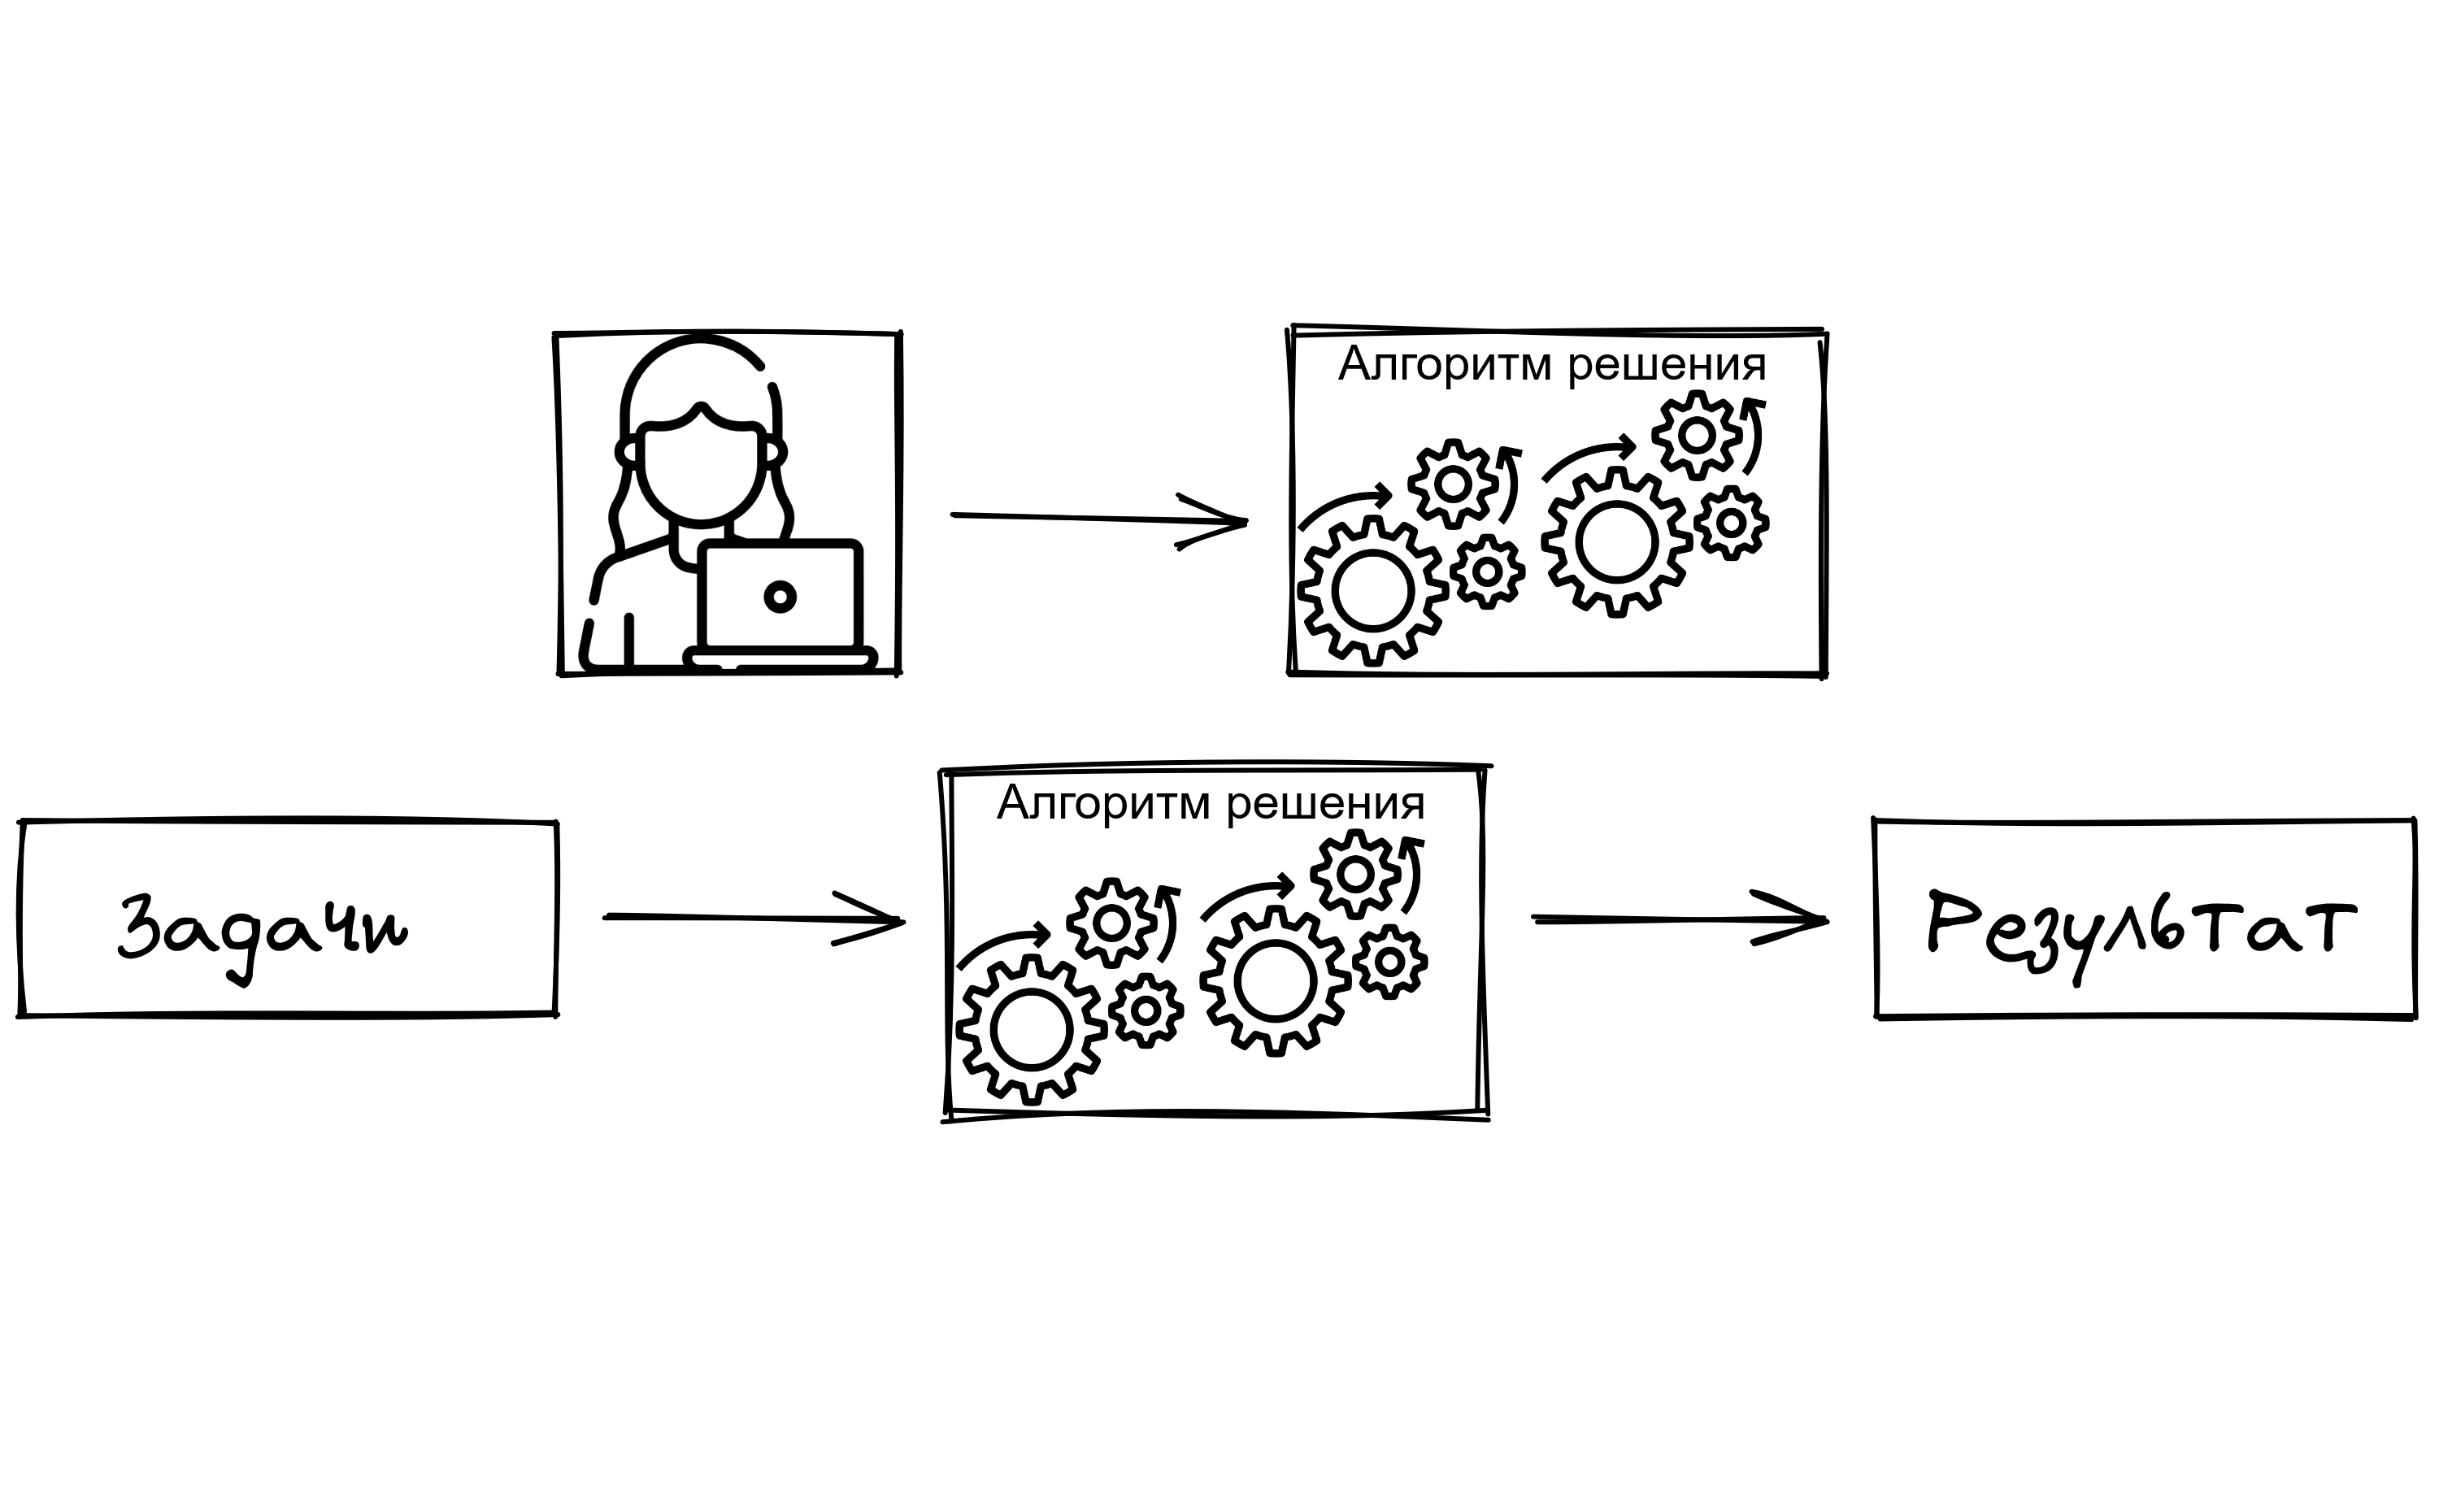
\includegraphics[width=\linewidth]{figures/fig40-swe-approach.jpg}
        \end{column}
        \pause
        \begin{column}{.49\linewidth}
            \centering
            Machine Learning
            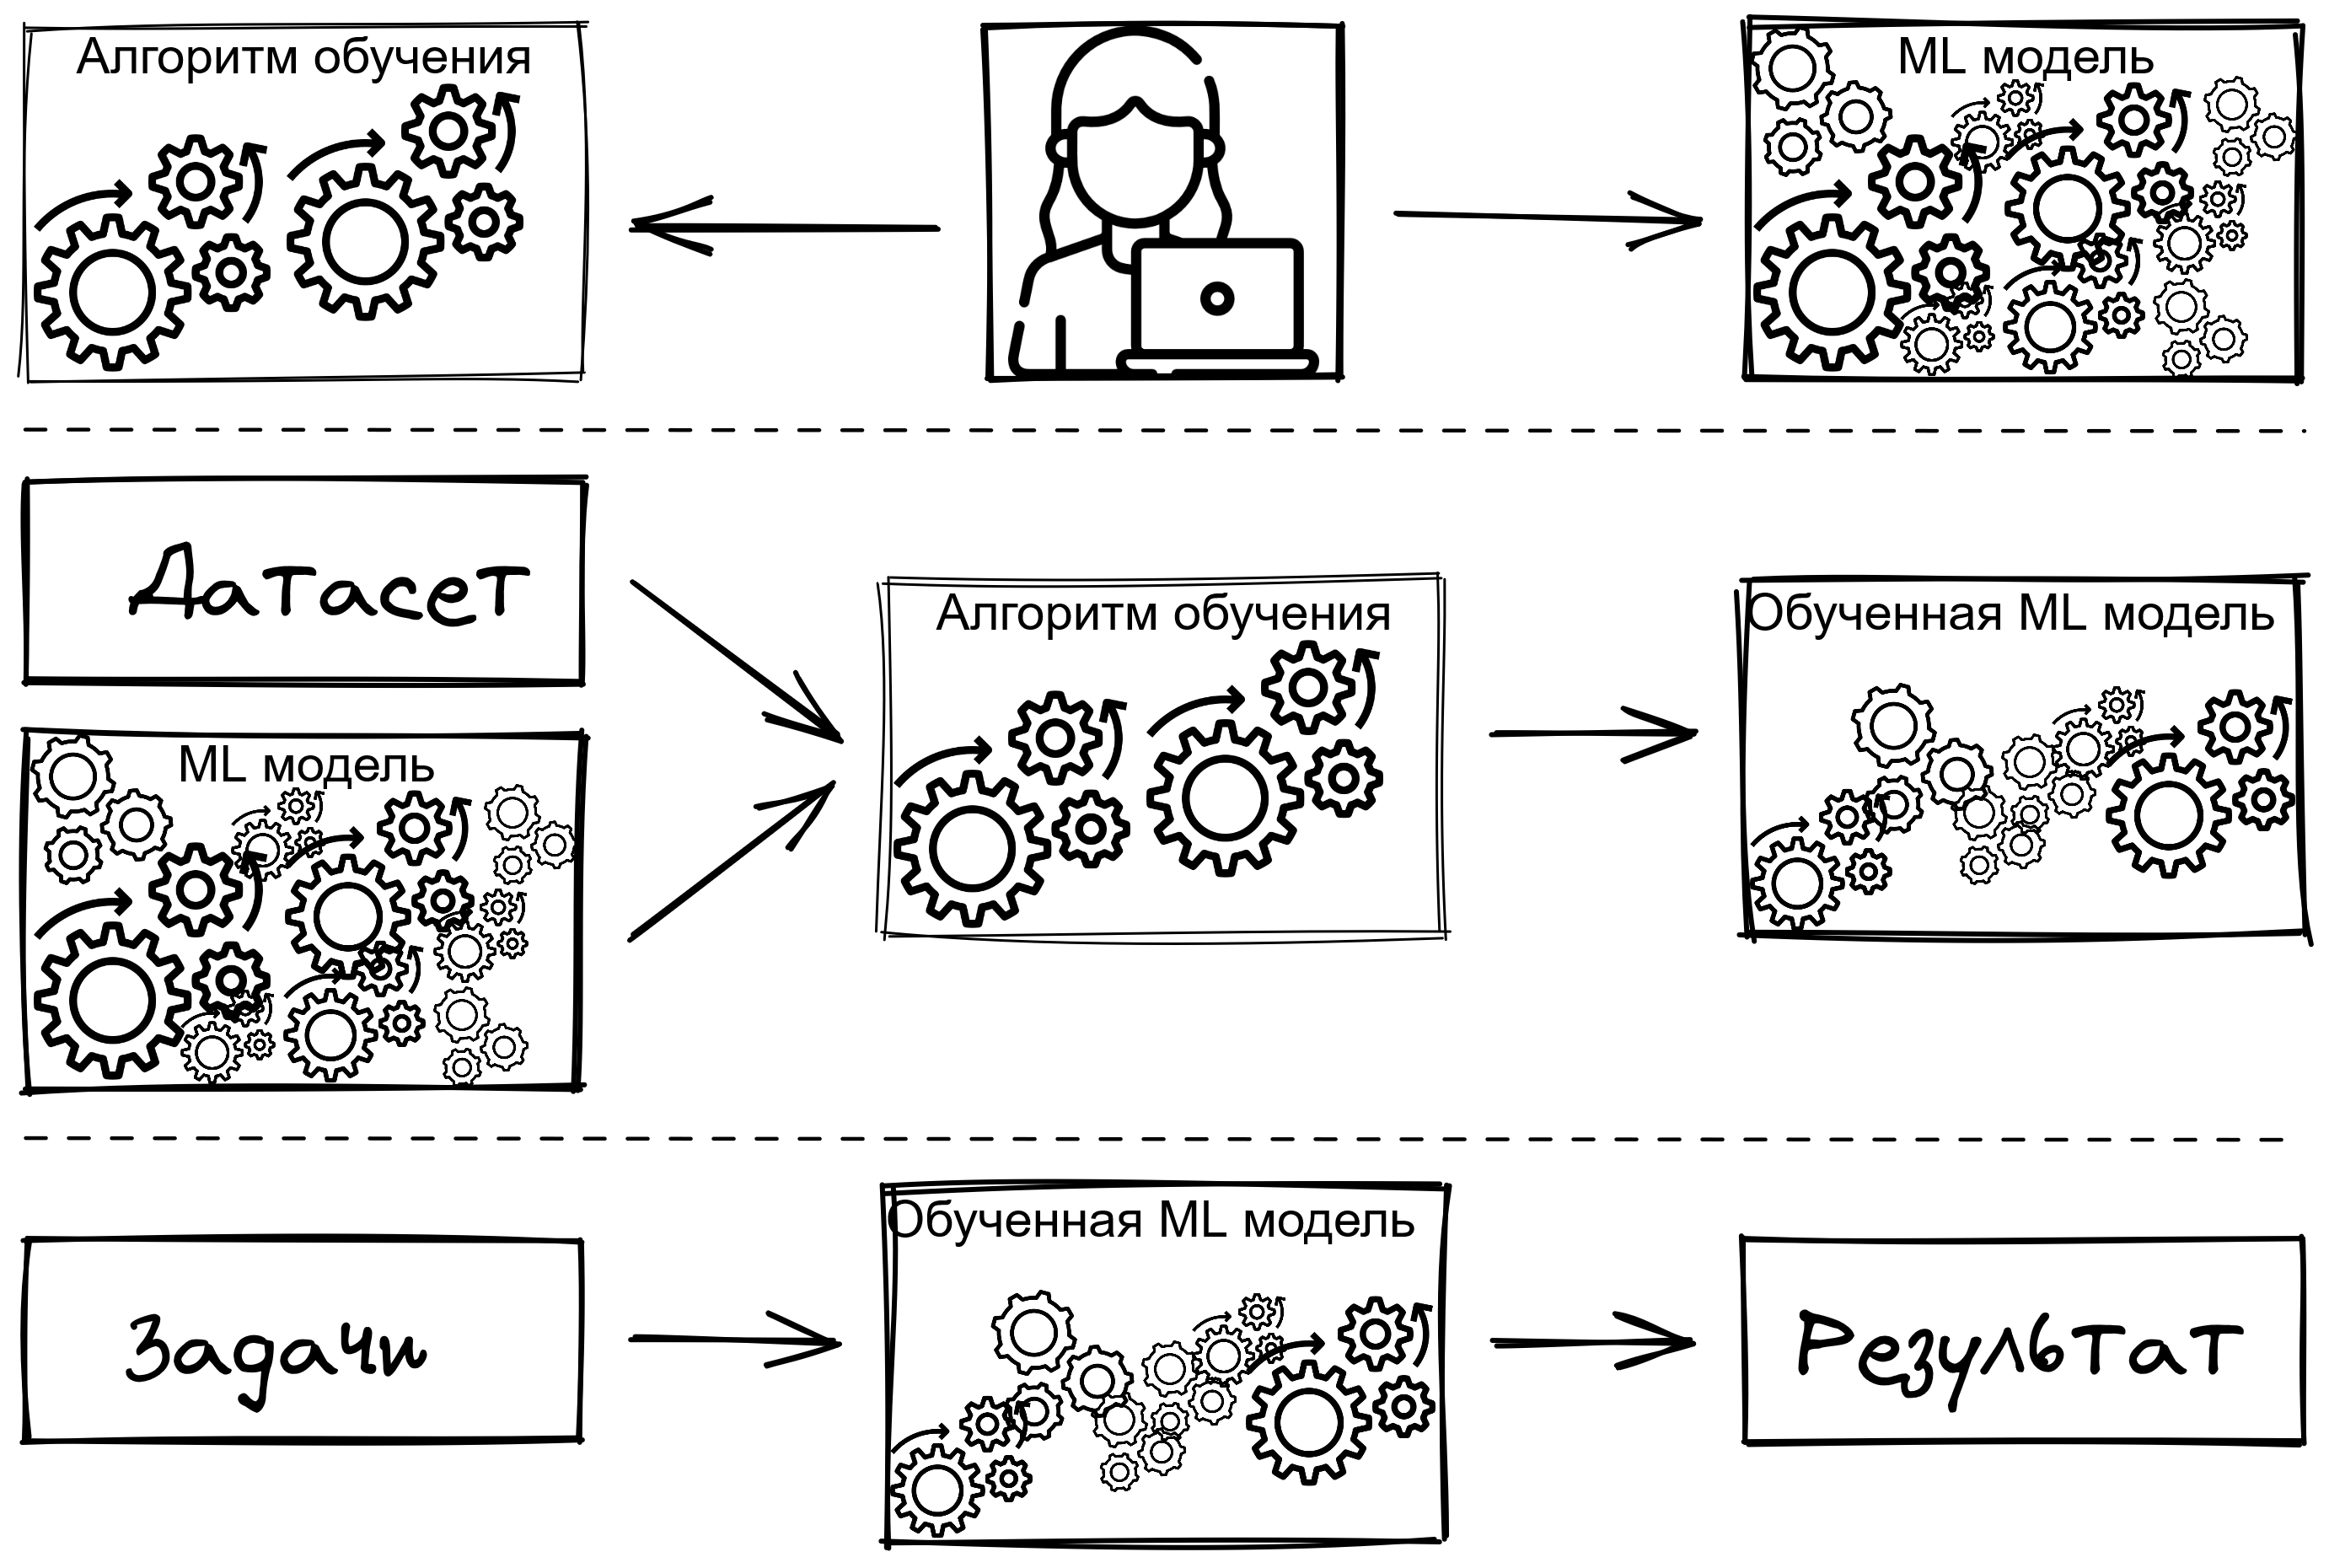
\includegraphics[width=\linewidth]{figures/fig41-ml-approach.jpg}
        \end{column}
    \end{columns}
\end{frame}

\begin{frame}{Когда применим ML?}
    Алгоритмы ML хорошо подходят в случаях, когда:
    \begin{outline}
        \1 мы не можем создать точный алгоритм решения задачи, потому что плохо понимаем
        лежащие в её основах процессы и \textbf{не можем построить} точную модель этих процессов
        \pause
        \1 или же модель есть, но ее полный расчет невозможен ввиду вычислительных
        ограничений (примеры --- квантовая химия (AlphaFold2), игра в го (AlphaZero))
        \pause
        \1 \textbf{но} при этом мы можем собрать \textbf{достаточное} количество данных с примерами
        решения задачи
    \end{outline}
\end{frame}

\begin{frame}{Когда применим ML?}
    \begin{outline}
        \1 Модели машинного обучения пытаются \textbf{восстанавливать закономерности} на
        основе \textbf{данных}, а не исходя из понимания природы или здравого смысла
        \1 ``Золотое'' правило машинного обучения
    \end{outline}
    \begin{center}
        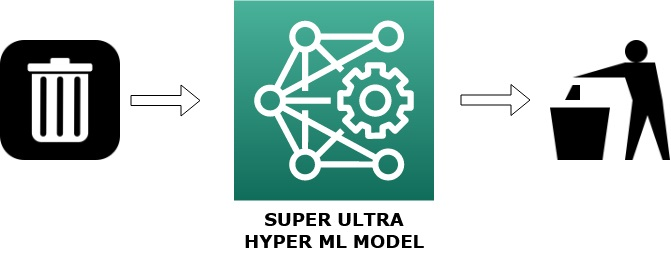
\includegraphics[width=.49\linewidth]{figures/fig42-golden-rule.jpg} \\
        garbade in --- garbage out
    \end{center}
\end{frame}

\begin{frame}{Почему применять ML сложно?}
    \begin{outline}
        \1 Машинное обучение находится на стыке матстатистики, computer science и
        вычислительной математики (численной оптимизации)
        \pause
        \1 ML алгоритмы являются статистическими по своей сути, поэтому их использование
        включает в себя допущение о ``стационарности'' (сохранении характеристик)
        задачи (отрицательный пример - предсказание курса акций)
        \pause
        \1 Модель учится на некоторой конечной выборке данных, а мы хотим чтобы она
        работала в будущем, на новых данных
        \pause
        \1 Специфичные проблемы: недообучение, переобучение, протечки, ...
        \1 Специфичные способы проверки корректности алгоритмов
    \end{outline}
\end{frame}

\begin{frame}{Если это не учитывать, то\ldots}
    \centering
    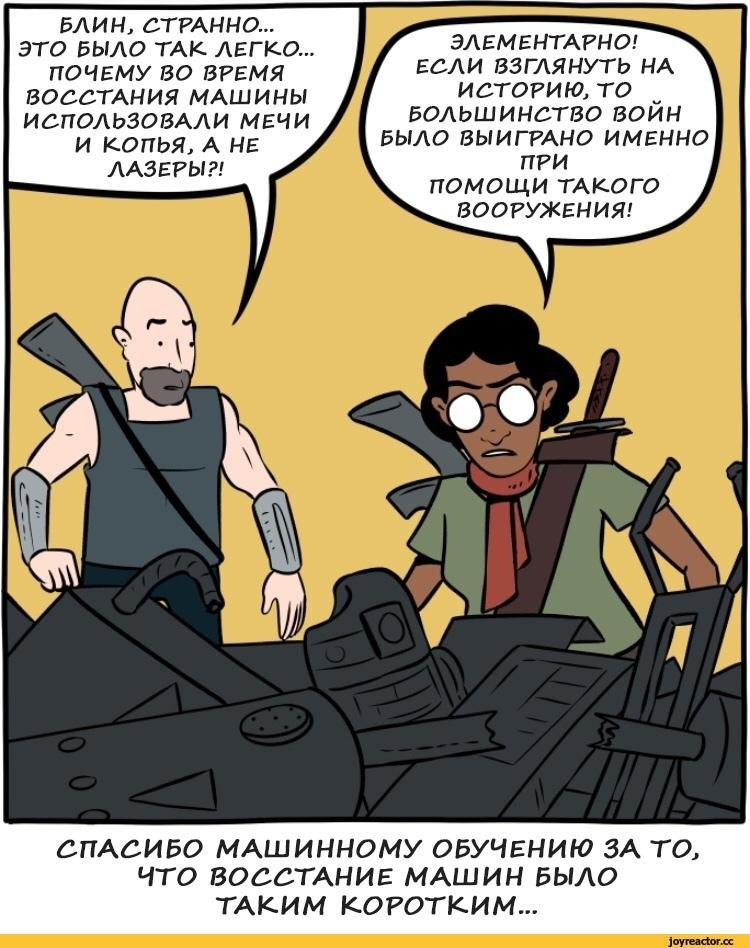
\includegraphics[width=.345\linewidth]{figures/fig43-ml-fuckup.jpg} \\
    \ldots результат часто получается примерно таким
\end{frame}

\begin{frame}{История исследований}
    \centering
    \includegraphics[width=\linewidth]{figures/fig44-research-history.jpg} \\
    82 года истории исследований AI
\end{frame}

\begin{frame}{Взлёт и падение модели перцептрона}
    \begin{columns}
        \begin{column}{.49\linewidth}
            \centering
            \includegraphics[width=.7\linewidth]{figures/fig45-rosenblatt.jpg} \\
            Фрэнк Розенблатт и первый в мире нейрокомпьютер (1958г.)
        \end{column}
        \pause
        \begin{column}{.49\linewidth}
            \centering
            \includegraphics[width=.52\linewidth]{figures/fig46-perceptrons.jpg} \\
            Книга, которая разрушила его работу (1969г.)
        \end{column}
    \end{columns}
\end{frame}

\begin{frame}{История исследований}
    \centering
    \includegraphics[width=\linewidth]{figures/fig44-research-history.jpg} \\
    82 года истории исследований AI
\end{frame}

\begin{frame}{Уроки истории}
    \large
    \begin{outline}
        \1 Искусственные нейросети были изобретены не несколько лет назад, а еще в 50-е
        \1 Со времени своего изобретения они прошли несколько пиков популярности и забвения
        \1 До 90-х область страдала от отсутствия эффективных методов обучения моделей
        \1 До середины 10-х ученые в области нейросетей (и шире, AI) были на``маргинальном'' положении
    \end{outline}

    Почему тогда сейчас нейронные сети и машинное обучение опять на хайпе?
\end{frame}

\begin{frame}{Наступил 2012 год}
    \centering
    \includegraphics[width=.85\linewidth]{figures/fig47-2012.jpg}
\end{frame}

\begin{frame}{Больше данных}
    \centering
    \includegraphics[width=\linewidth]{figures/fig48-internet-growth.jpg}
\end{frame}

\begin{frame}{Больше размеченных данных: ImageNet}
    \centering
    \includegraphics[width=\linewidth]{figures/fig49-imagenet.jpg}
\end{frame}

\begin{frame}{Больше размеченных данных: ImageNet}
    \centering
    \includegraphics[width=.97\linewidth]{figures/fig50-imagenet-overview.jpg}
\end{frame}

\begin{frame}{Больше размеченных данных: ImageNet}
    \begin{columns}[T]
        \begin{column}{.6\linewidth}
            \begin{outline}
                \1 C 2010 года проводится ILSVRC --- ImageNet Large Scale Visual
                Recognition Competition
                \1 Это соревнование, помимо открытого доступа к большому датасету
                ImageNet, дало научному сообществу простой способ сравнивать
                различные модели, что сильно ускорило прогресс в области компьютерного зрения,
                а подобный подход перенесли и в другие области (текст, звук)
            \end{outline}
        \end{column}
        \begin{column}{.39\linewidth}
            \centering
            \includegraphics[width=\linewidth]{figures/fig51-fei-fei-li.jpg} \\
            Dr. Fei-Fei Li
        \end{column}
    \end{columns}
\end{frame}

\begin{frame}{Много данных --- тоже проблема}
    \begin{columns}
        \begin{column}{.49\linewidth}
            \centering
            \includegraphics[width=.55\linewidth]{figures/fig52-waiting.jpg} \\
            70е: нет эффективных алгоритмов, нет данных, нет мощностей
        \end{column}
        \begin{column}{.49\linewidth}
            \centering
            \includegraphics[width=.7\linewidth]{figures/fig53-waiting.jpg} \\
            00е: данных подросло, но расчеты будут идти вечность
        \end{column}
    \end{columns}
\end{frame}

\begin{frame}{Геймеры спасают науку о данных}
    \centering
    \includegraphics[width=.83\linewidth]{figures/fig54-gamer-girl.jpg}
\end{frame}

\begin{frame}{GPU - Graphics Processing Unit}
    \centering
    \includegraphics[width=.74\linewidth]{figures/fig55-gpus.jpg}
\end{frame}

\begin{frame}{GPUs: конкуренция --- это прекрасно}
    \begin{columns}
        \begin{column}{.49\linewidth}
            \centering
            \includegraphics[width=\linewidth]{figures/fig56-nvidia.jpg}
        \end{column}
        \begin{column}{.49\linewidth}
            \centering
            \includegraphics[width=\linewidth]{figures/fig57-amd.jpg}
        \end{column}
    \end{columns}
\end{frame}

\begin{frame}{GPU vs. CPU}
    \centering
    \includegraphics[width=.92\linewidth]{figures/fig58-cpu-gpu.jpg}
\end{frame}

\begin{frame}{Ученые любят GPU}
    \centering
    \includegraphics[width=\linewidth]{figures/fig59-matrices.jpg}
\end{frame}

\begin{frame}{Что произошло в 2012 году}
    \begin{outline}
        \1 Alex Krizhevsky принял участие в ILSVRC, взяв в качестве алгоритма вариацию
        нейронной сети, представленную еще в 1989 году
        \1 Он обучил ее на данных ImageNet используя 2 GPU NVIDIA GTX 580
        \1 Эта модель обошла конкурентов на более чем 10.8\% п. п.
        \1 Начиная с 2012 года в ILSVRC побеждали только нейросетевые алгоритмы
        \1 Стало понятно, что нейросетевые модели забыты незаслуженно и им просто нужно
        больше данных и вычислительных мощностей, чтобы презвойти любые другие алгоритмы
        обработки изображений
    \end{outline}
\end{frame}

\begin{frame}{Итоги DL-революции 2012 года}
    \centering
    \includegraphics[width=.75\linewidth]{figures/fig60-ilsvrc-results.jpg}
\end{frame}

\begin{frame}{Итоги DL-революции 2012 года}
    \centering
    \includegraphics[width=.8\linewidth]{figures/fig61-nips.jpg} \\
    Количество принятых статей на конференцию NeurIPS
\end{frame}

\begin{frame}{Из 2012 в 2024}
    \centering
    \includegraphics[width=.6\linewidth]{figures/fig62-dl-everywhere.jpg}
\end{frame}

\begin{frame}{Суть машинного обучения}
    \centering
    \includegraphics[width=.35\linewidth]{figures/fig63-ml-core.jpg} \\
    К концу курса вы сможете лучше понять этот мем
\end{frame}

\end{document}
